\documentclass[11pt,a4paper]{article}

\usepackage[margin=1in]{geometry}
\usepackage{amsmath,amssymb,amsfonts,bm,mathtools}
\usepackage{booktabs}
\usepackage{graphicx}
\usepackage{float}
\usepackage{caption}
\usepackage{microtype}
\usepackage{enumitem}
\usepackage{hyperref}
\usepackage{xcolor}

\hypersetup{
  colorlinks=true,
  linkcolor=blue!50!black,
  urlcolor=blue!60!black,
  citecolor=blue!50!black
}

\graphicspath{{figs/}}

\newcommand{\Einc}{E_{\mathrm{inc}}}
\newcommand{\Eloc}{E_{\mathrm{loc}}}
\newcommand{\Escat}{E_{\mathrm{scat}}}
\newcommand{\om}{\omega}
\newcommand{\alpm}{\alpha_m}
\newcommand{\alpeff}{\alpha_{\mathrm{eff}}}
\newcommand{\Araw}{A_{\mathrm{raw}}}
\newcommand{\Adiss}{A_{\mathrm{diss}}}
\newcommand{\Ainc}{A_{\mathrm{inc}}}
\newcommand{\sigmol}{\sigma_{\mathrm{mol}}}
\newcommand{\re}[1]{\operatorname{Re}[#1]}
\newcommand{\im}[1]{\operatorname{Im}[#1]}

\title{Getting Spectra from PlasMol}
\author{}
\date{\today}

\begin{document}
\maketitle

\tableofcontents
\newpage

% =============================================================================
\section{Parallel orientation and the three recorded series}
\label{sec:setup}
% =============================================================================

\noindent
This PlasMol calculation is hybrid NP + molecule in the parallel geometry.
A $25\mathrm{nm}$ Au sphere sits at the origin.
The Na atom is on the $+x$ axis at $d=26.451\mathrm{nm}$ (gap $1.451\mathrm{nm}$).
The source is a transverse plane wave arranged so that the driving field at the atom is along the line from the nanoparticle center to the atom (Figure~\ref{fig:geom}).
RT-TDDFT (LC-$\omega$PBE / $6$-$31$G$^{\ast}$, IP-tuned range-separation $\omega=0.339181$, static CAP) is advanced under the length-gauge coupling to the Meep field sampled at the atomic site.\\

\begin{figure}[H]
  \centering
  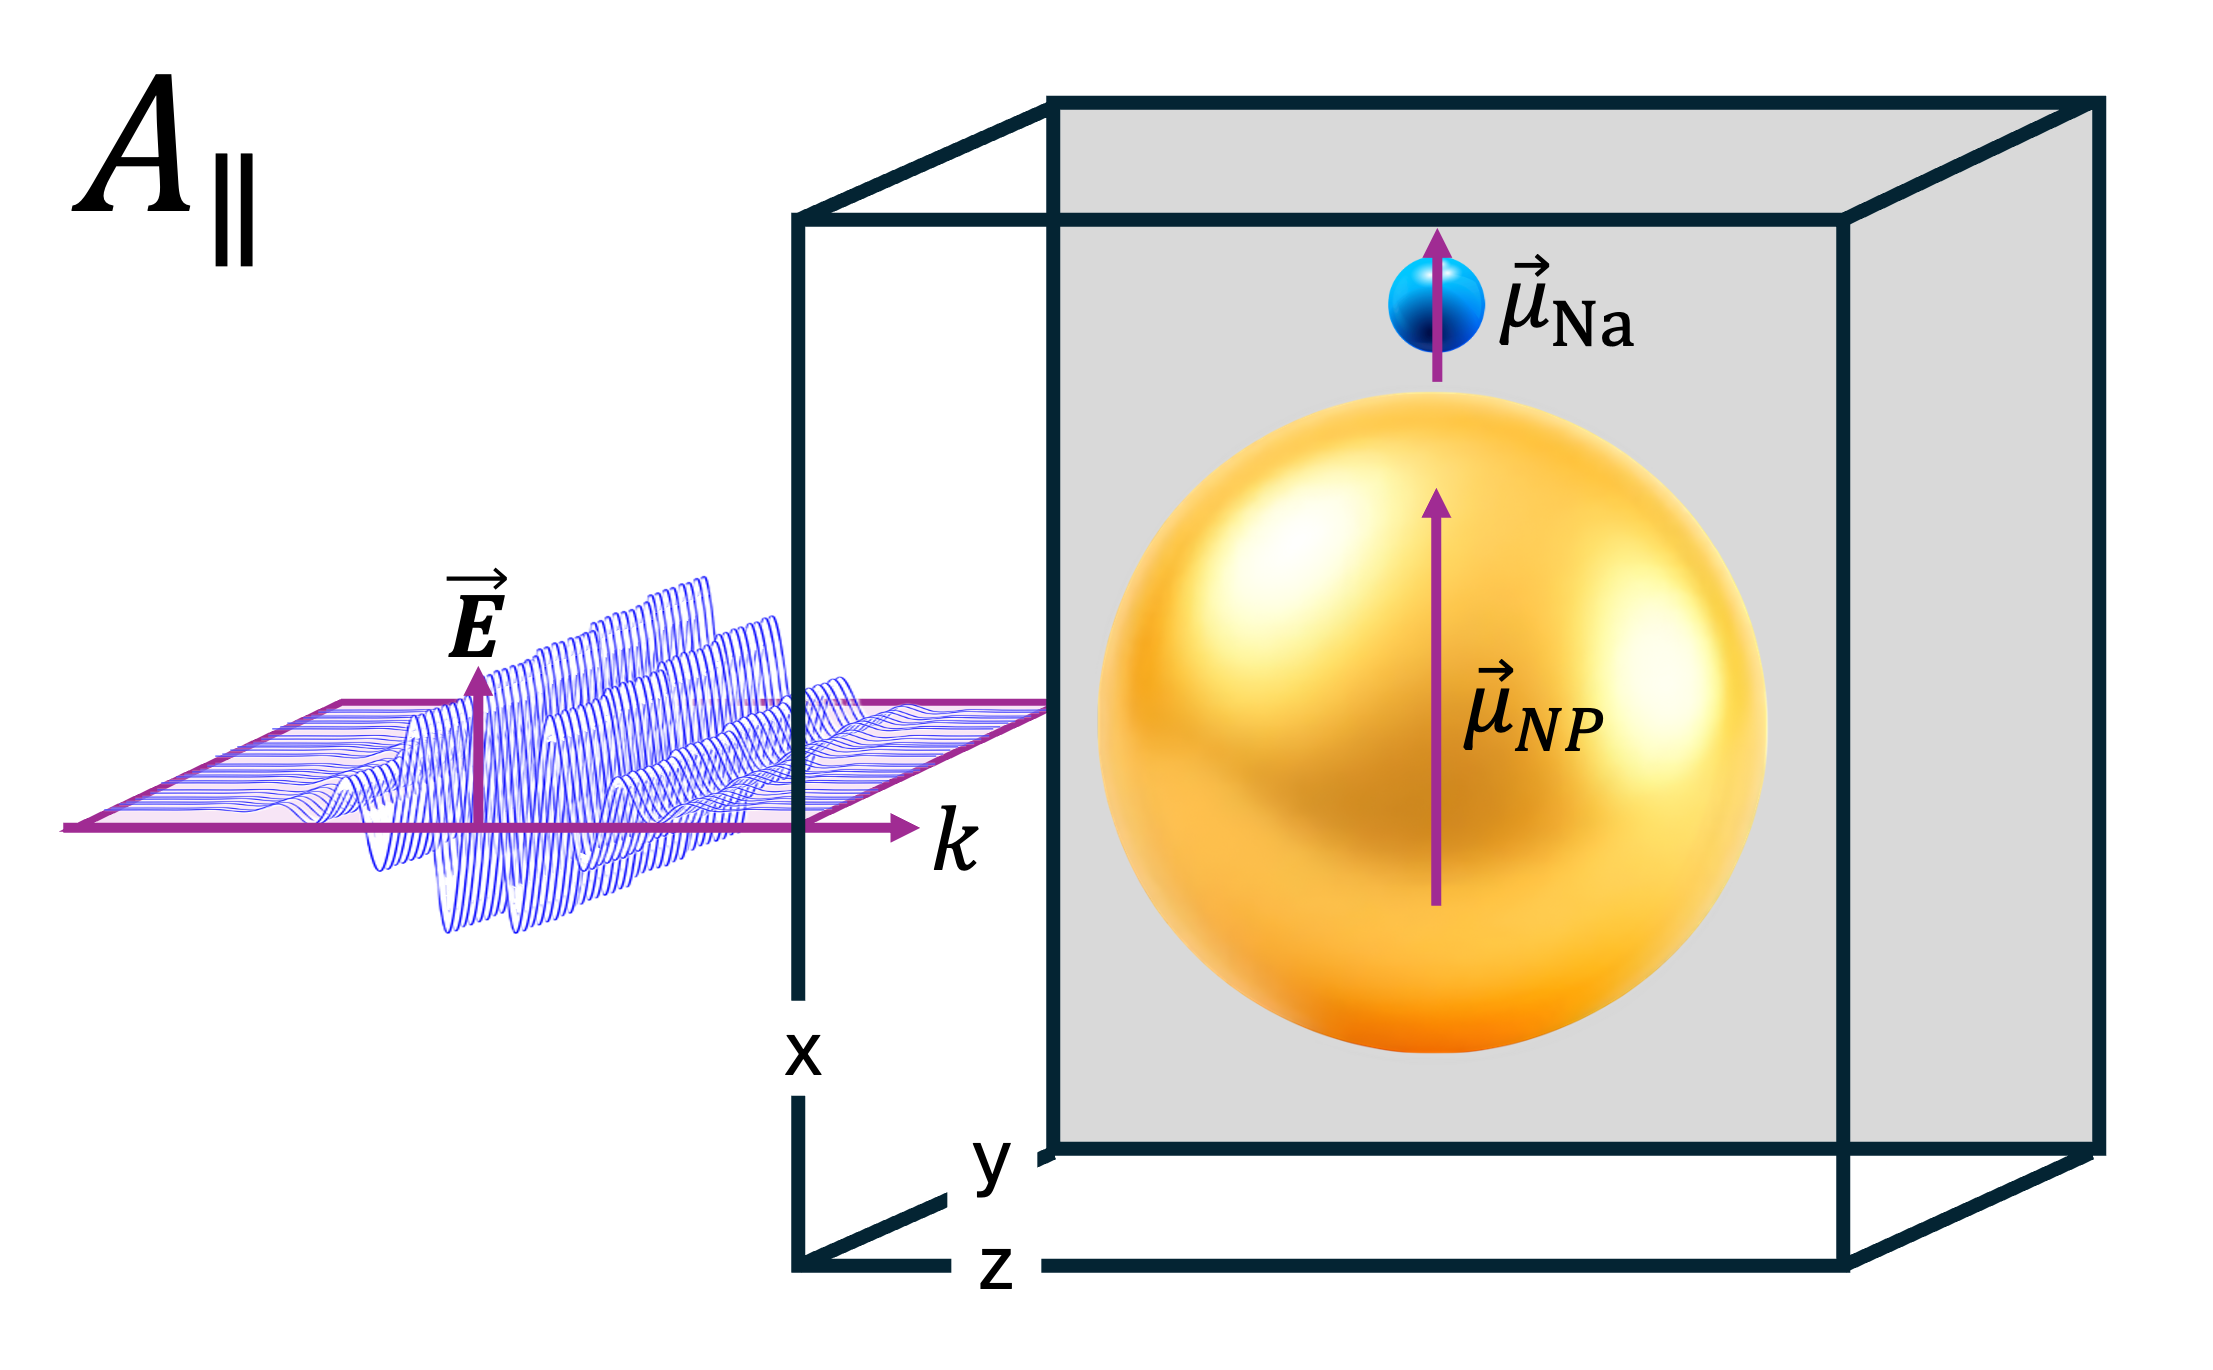
\includegraphics[width=0.88\textwidth]{parallel_geometry.png}
  \caption{Parallel (radial) orientation, from the PlasMol documentation. The incident wave is transverse ($\mathbf{k}\perp\mathbf{E}$). Both $\boldsymbol{\mu}_{\mathrm{NP}}$ and $\boldsymbol{\mu}_{\mathrm{Na}}$ lie along the nanoparticle--molecule axis $\hat{\mathbf{r}}$. In the production job the atom is on the $+x$ axis at $d=26.45\mathrm{nm}$ (gap $1.45\mathrm{nm}$). Time traces at the Na site are in Figure~\ref{fig:series-time}.}
  \label{fig:geom}
\end{figure}

\noindent
Every production run writes three real functions of time at the molecular location:
\begin{itemize}[leftmargin=1.6em]
  \item $\Eloc(t)$: the electric field felt by the molecule (nanoparticle scattering included).
  \item $\mu(t)$: the induced dipole of the \emph{molecule} (RT-TDDFT).
  \item $\Einc(t)$: the electric field at the same sample point in a vacuum reference run (same source, no nanoparticle, no molecule).
\end{itemize}
In the frequency domain the local field is the incident wave plus whatever the gold sphere (and, weakly, the molecule reflecting off the sphere) scatter,
\begin{equation}
  \Eloc(\om)
  =
  \Einc(\om)+\Escat(\om).
  \label{eq:split}
\end{equation}
The three hybrid traces are shown in Figure~\ref{fig:series-time}.\\

\begin{figure}[H]
  \centering
  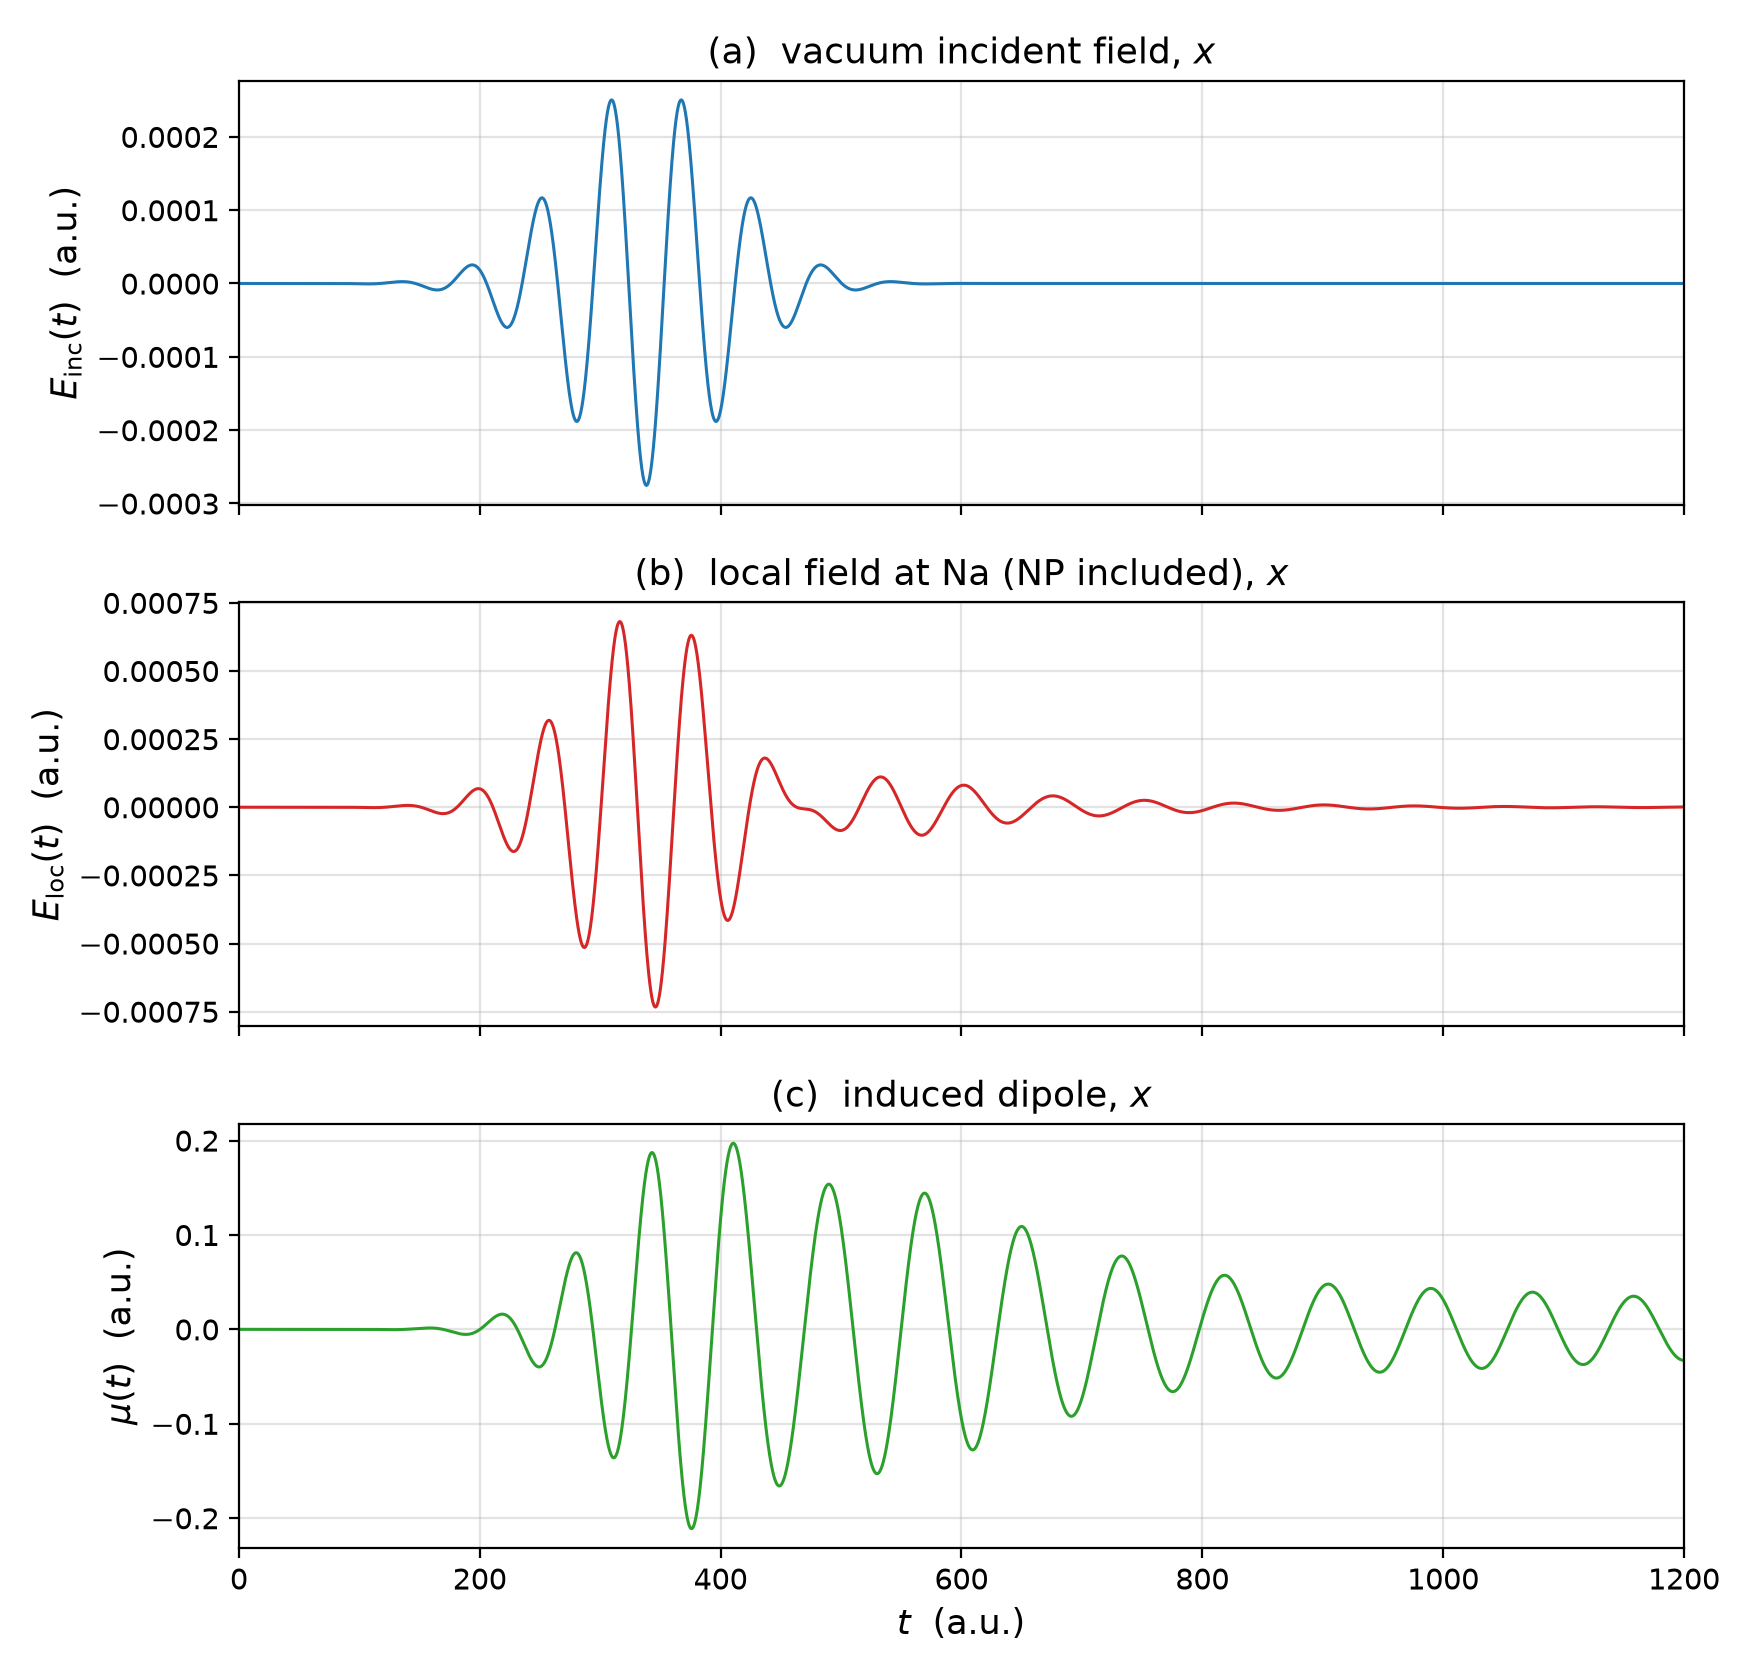
\includegraphics[width=0.92\textwidth]{series_time.png}
  \caption{Driven ($x$) components through the arrival of the Meep pulse. (a)~$\Einc(t)$. (b)~$\Eloc(t)$, larger and ringing after the vacuum pulse has gone. (c)~$\mu(t)$, which continues to oscillate after both fields have died until about \( t=4000 \text{ a.u.} \).}
  \label{fig:series-time}
\end{figure}

% =============================================================================
\section{Fourier transforms and linear response}
\label{sec:fourier}
% =============================================================================

\subsection{Beginning equations}
\noindent
Frequency domain spectra are formed with the same discrete transform PlasMol uses,
\begin{equation}
  f(\om_k)
  =
  \Delta t\sum_{n=0}^{N-1} f(t_n)e^{-\mathrm{i}\om_k t_n},
  \qquad
  \om_k
  =
  \frac{2\pi k}{N\Delta t}.
  \label{eq:dft}
\end{equation}
Even though the three traces collected are real, their transforms are nevertheless complex (Figure~\ref{fig:series-ft}).

\begin{figure}[H]
  \centering
  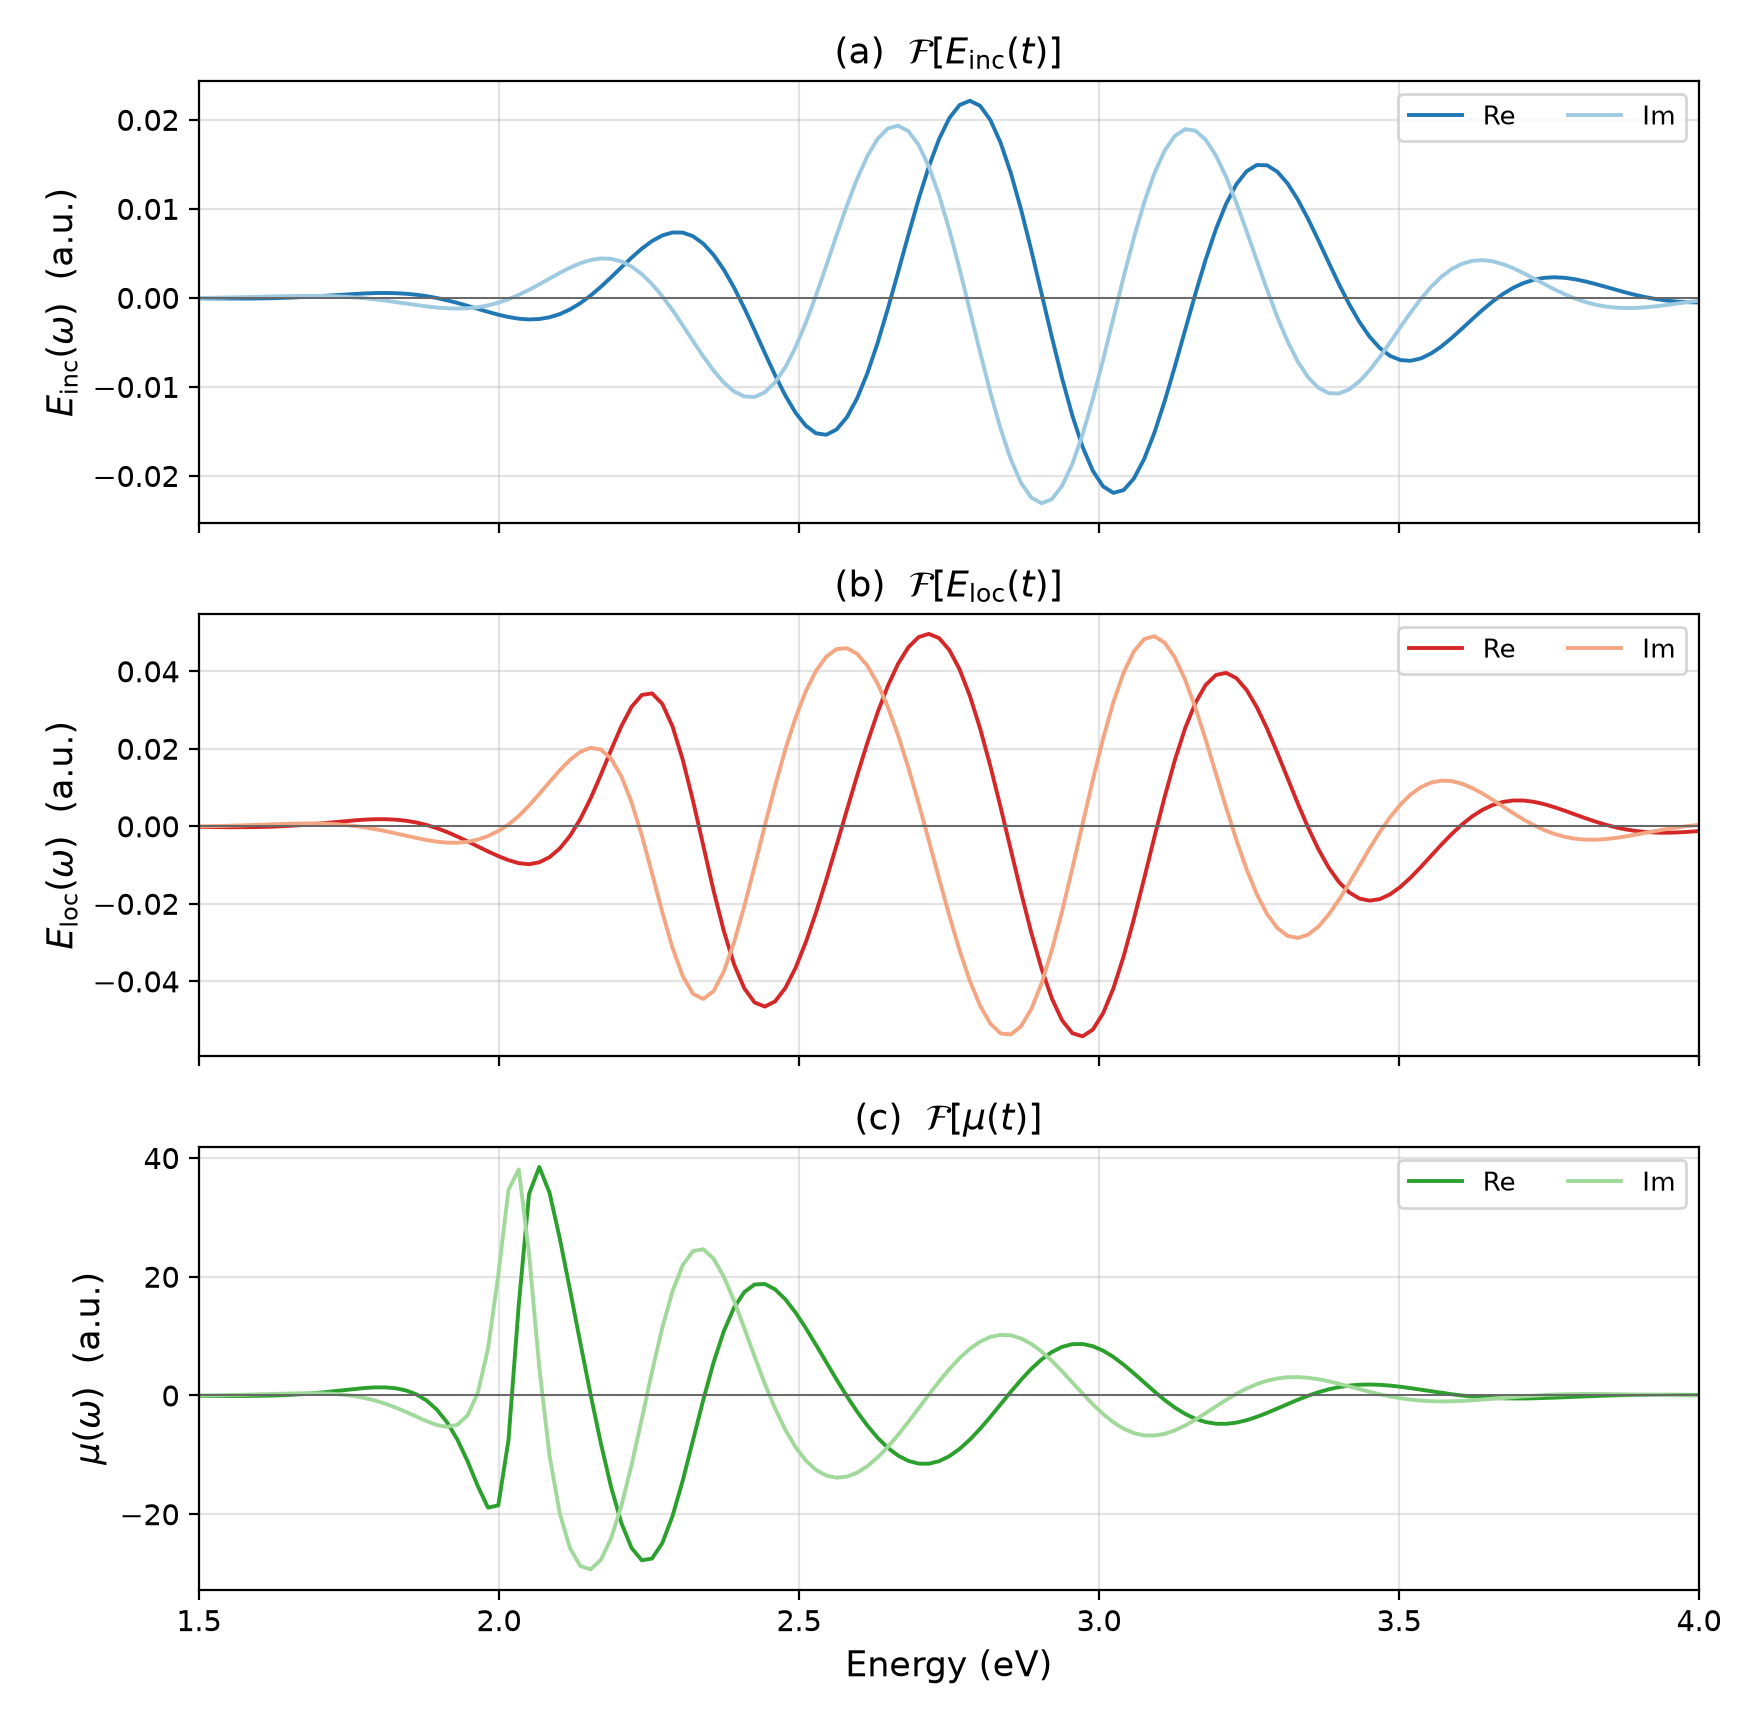
\includegraphics[width=0.92\textwidth]{series_fourier.png}
  \caption{Real and imaginary parts of $\Einc(\om)$, $\Eloc(\om)$, and $\mu(\om)$. The DFT oscillates because the time-dependent fields are not centered at $t=0$.}
  \label{fig:series-ft}
\end{figure}

\noindent
Taking the magnitude of the DFTs in Figure~\ref{fig:series-ft} gives what is traditionally viewed as an energy spectrum.
Figure~\ref{fig:Einc-mod} is that construction for the incident field: $\lvert\Einc(\om)\rvert$ is the envelope of the Meep pulse, peaked near $2.84\,\mathrm{eV}$.\\

\begin{figure}[H]
  \centering
  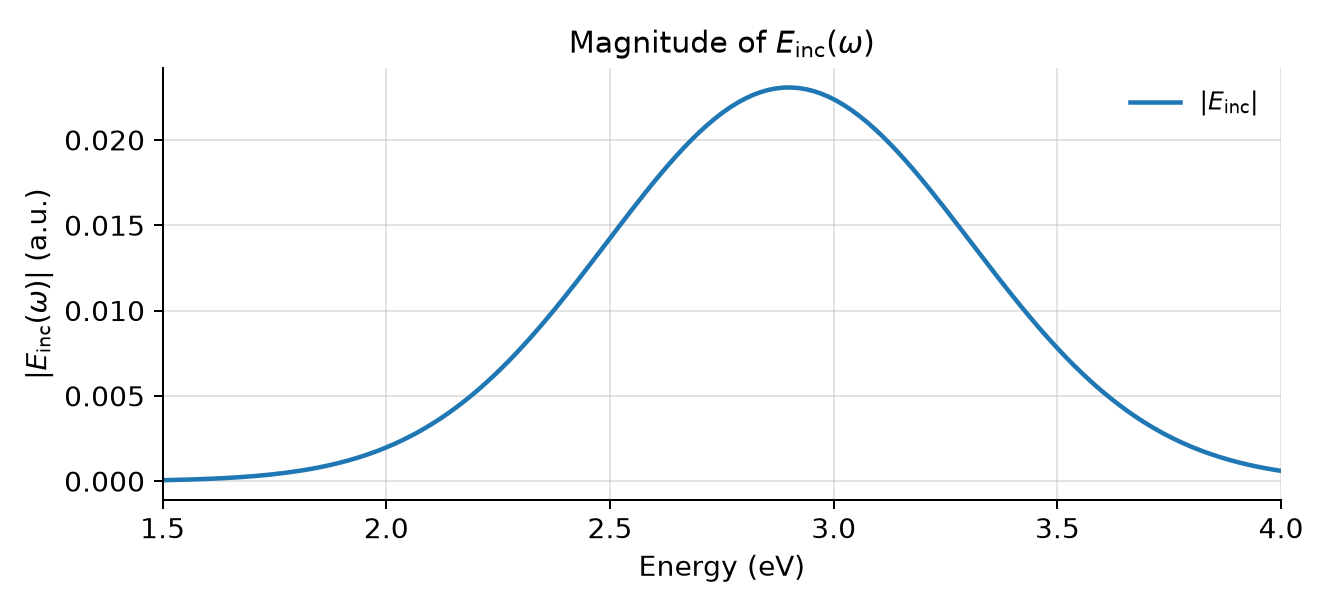
\includegraphics[width=0.78\textwidth]{Einc_modulus.png}
  \caption{Magnitude of $\Einc(\om)$ from the vacuum reference. This is the usual energy spectrum of the incident pulse; the delay phase that oscillates in Figure~\ref{fig:series-ft} does not appear in $\lvert\Einc\rvert$.}
  \label{fig:Einc-mod}
\end{figure}

\noindent
If the simulation were centered around $t=0$, the Fourier transform would not have the pulsing seen in Figure~\ref{fig:series-ft}.
Figure~\ref{fig:Einc-centered} is an illustrative example, not a production hybrid run: the same vacuum $\Einc$ with its peak shifted to the origin.
The real part is then a smooth envelope and the imaginary part is nearly gone; $\lvert\Einc(\om)\rvert$ is unchanged by the shift.\\

\begin{figure}[H]
  \centering
  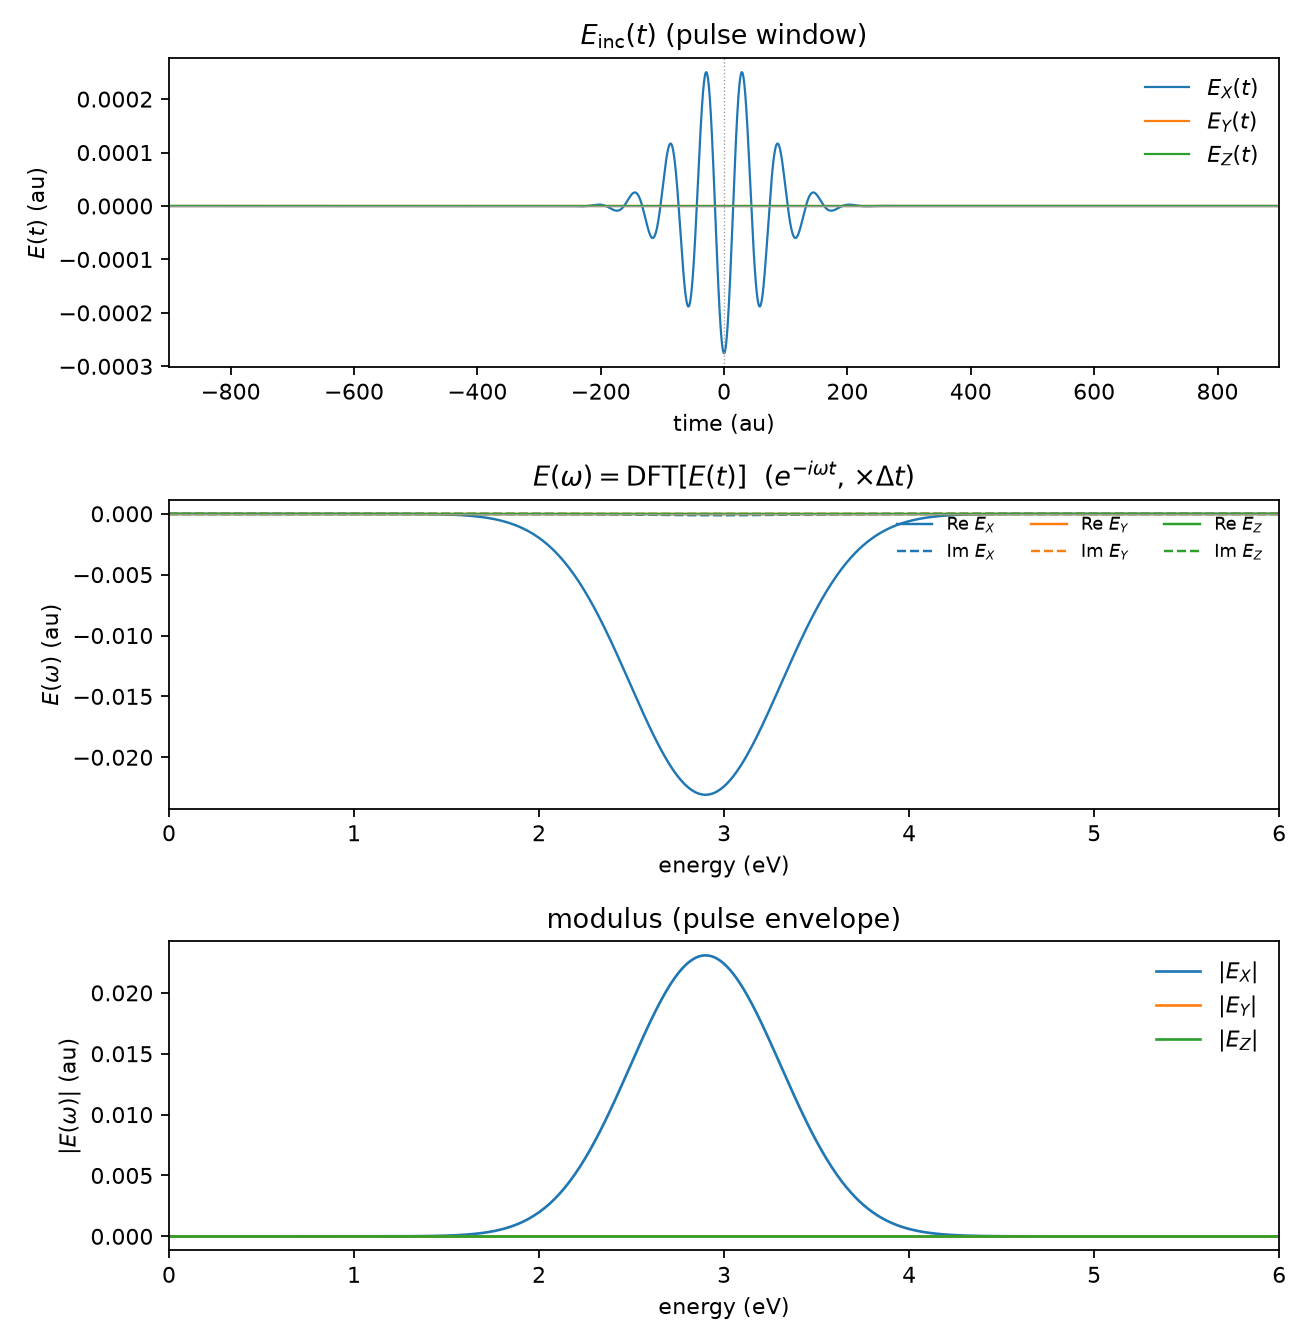
\includegraphics[width=0.88\textwidth]{field_e_ref_centered_ft.png}
  \caption{Illustrative example. The vacuum incident pulse of Figure~\ref{fig:series-time} recentered at $t=0$. Top: time trace. Middle: real and imaginary parts of the DFT; the delay pulsing of Figure~\ref{fig:series-ft} is absent. Bottom: $\lvert\Einc(\om)\rvert$, the same envelope as Figure~\ref{fig:Einc-mod}.}
  \label{fig:Einc-centered}
\end{figure}

% =============================================================================
\section{Power of the molecule}
\label{sec:phasors}
% =============================================================================
\subsection{Instantaneous power}

\noindent
The instantaneous power delivered to a classical dipole by the electric field at its location is
\begin{equation}
  P(t)
  =
  \dot{\mu}(t)\Eloc(t).
  \label{eq:Pt}
\end{equation}
This is the rate at which the local field does work on the oscillating charge distribution.
Ideally, the energy that enters~\eqref{eq:Pt} would leave the electromagnetic field and sit in the atom or be subsequently removed by the CAP (though that is not technically the case within the discrete nature of PlasMol).\\

\noindent
For future steps, it is useful to write a real field in phasor notation,
\begin{equation}
  E(t)
  =
  \re{\tilde E e^{-\mathrm{i}\om t}},
  \qquad
  \mu(t)
  =
  \re{\tilde\mu e^{-\mathrm{i}\om t}},
  \label{eq:phasor}
\end{equation}
with independent phasors 
\begin{equation}
  \tilde E
  =
  \lvert E\rvert e^{\mathrm{i}\varphi_E},
  \qquad
  \tilde\mu
  =
  \lvert\mu\rvert e^{\mathrm{i}\varphi_{\mu}}.
  \label{eq:phasor-amp}
\end{equation}
Linear response of the molecule is always to the field at its location,
\begin{equation}
  \mu(\om)
  =
  \alpm(\om)\Eloc(\om),
  \label{eq:mu}
\end{equation}
or, in the same phasors, $\tilde\mu=\alpm\tilde E_{\mathrm{loc}}$.
Here $\alpm$ is the molecular polarizability of the RT-TDDFT model, CAP included.
The two phases are not assumed equal: if they were, $\mu(t)$ would be in phase with $E(t)$ and the cycle-averaged power would vanish.
The physical field is always the real part.
Under~\eqref{eq:phasor} the time derivative is

\begin{equation}
  \dot{\mu}(t)
  =
  \re{-\mathrm{i}\om\tilde\mu e^{-\mathrm{i}\om t}}.
  \label{eq:mudot}
\end{equation}

\subsection{Cycle-averaged power}

\noindent Instantaneous power oscillates. Half the cycle the field does work on the dipole; the other half the dipole does work on the field. That sloshing is reactive energy, stored and returned every period. It is not absorption. In order to get absorption, we want to see the net transfer of power, leftover after many cycles:
\begin{equation*}
  \begin{aligned}
    \bar{P}&=\frac{1}{T} \int_0^T P(t) dt\\
    &=\frac{1}{T} \int_0^T \dot{\mu}(t)\Eloc(t) dt\\
    &=\frac{1}{T} \int_0^T \re{-\mathrm{i}\om\tilde\mu e^{-\mathrm{i}\om t}} \re{\tilde{E}_{\mathrm{loc}} e^{-\mathrm{i}\om t}} dt
  \end{aligned}
\end{equation*}

\noindent
Write $A=\re{\tilde Ae^{-\mathrm{i}\om t}}$ and $B=\re{\tilde Be^{-\mathrm{i}\om t}}$.
Without loss of generality,
\begin{equation}
  A = \re{\tilde Ae^{-\mathrm{i}\om t}}
  =
  \tfrac12\bigl(\tilde Ae^{-\mathrm{i}\om t}+\tilde A^{\ast}e^{\mathrm{i}\om t}\bigr),
\end{equation}
so the product is
\begin{equation}
  AB
  =
  \tfrac14\bigl(
    \tilde A\tilde Be^{-2\mathrm{i}\om t}
    +\tilde A\tilde B^{\ast}
    +\tilde A^{\ast}\tilde B
    +\tilde A^{\ast}\tilde B^{\ast}e^{2\mathrm{i}\om t}
  \bigr).
  \label{eq:ABprod}
\end{equation}
The double-frequency terms average to zero over one period $T=2\pi/\om$ and both $\tilde A$ and $\tilde B$ are time independent.
The cycle average is therefore
\begin{equation}
  \overline{AB}
  =
  \frac{1}{T}\int_{0}^{T} AB\,dt
  =
  \frac{1}{T} \left( \tfrac14\bigl(\tilde A\tilde B^{\ast}+\tilde A^{\ast}\tilde B\bigr) \right) T
  =
  \tfrac12\re{\tilde A\tilde B^{\ast}}
  \label{eq:ABavg}
\end{equation}
where the following identity was used:
\begin{equation}
  CD^* + C^* D
  =
  CD^* + (CD^*)^* = 2 \operatorname{Re}[CD^*].
\end{equation}

\noindent
Identify $A=\re{-\mathrm{i}\om\tilde\mu e^{-\mathrm{i}\om t}} \implies \tilde A=-\mathrm{i}\om\tilde\mu$ and $B=\re{\tilde E_{\mathrm{loc}} e^{-\mathrm{i}\om t}} \implies \tilde B=\tilde E_{\mathrm{loc}}$.
Then
\begin{equation}
  \overline{P}
  =
  \tfrac12\re{(-\mathrm{i}\om\tilde\mu)\tilde E_{\mathrm{loc}}^{\ast}}.
  \label{eq:Pbar-Re}
\end{equation}
For real $\om$ one has $\re{(-\mathrm{i}z)}=\im{z}$, and~\eqref{eq:Pbar-Re} becomes
\begin{equation}
  \overline{P}
  =
  \frac{\om}{2}
  \im{\tilde\mu\tilde E_{\mathrm{loc}}^{\ast}}.
  \label{eq:Pbar}
\end{equation}
Inserting~\eqref{eq:mu} and using $\Eloc\Eloc^{\ast}=\lvert\Eloc\rvert^{2}\in\mathbb{R}$ gives
\begin{equation}
  \overline{P}
  =
  \frac{\om}{2}
  \im{\alpm}
  \lvert\tilde E_{\mathrm{loc}}\rvert^{2}.
  \label{eq:Pbar-alpha}
\end{equation}

\noindent
The Meep source is not a single harmonic.
Linearity of~\eqref{eq:mu} means each Fourier component of $\Eloc$ drives its own $\mu(\om)$ with its own $\alpm(\om)$.
The same bilinear form, evaluated on the DFTs~\eqref{eq:dft}, is the spectral density of the work~\eqref{eq:Pt}.
Thus,
\begin{equation}
  \overline{P}(\om)
  =
  \frac{\om}{2}
  \im{\mu(\om)\Eloc^{\ast}(\om)}
  =
  \frac{\om}{2}
  \im{\alpm(\om)}
  \lvert\Eloc(\om)\rvert^{2}.
  \label{eq:Pbar-w}
\end{equation}

\subsection{\texorpdfstring{Dissipated-power spectrum $\Adiss$}{Dissipated-power spectrum A\_diss}}
\label{sec:Adiss}

\noindent
Equation~\eqref{eq:Pbar-w} is already the dissipated-power spectrum.
To plot it next to a polarizability-like curve we give it the same $4\pi\om/c$ dressing used later for a plane-wave cross section, and the same DFT sign flip that turns a physical absorption peak upward,
\begin{equation}
  \Adiss(\om)
  =
  -\frac{4\pi\om}{c}
  \im{\mu(\om)\Eloc^{\ast}(\om)}.
  \label{eq:Adiss}
\end{equation}

\noindent
Figure~\ref{fig:Adiss} is~\eqref{eq:Adiss} for the hybrid job and for isolated Na.
The hybrid curve has one molecular peak at $2.05\,\mathrm{eV}$ and a shoulder near $2.2\,\mathrm{eV}$ from $\lvert\Eloc(\om)\rvert^{2}$ (plasmon plus the Meep pulse).\\

\noindent
Isolated $\Adiss$ uses the same formula, but there is no nanoparticle, so the field at the atom is the incident pulse, $\mu^{\mathrm{iso}}=\alpm\Einc$.
Equation~\eqref{eq:Adiss} therefore collapses to
\begin{equation}
  \Adiss^{\mathrm{iso}}(\om)
  =
  -\frac{4\pi\om}{c}\,
  \im{\mu^{\mathrm{iso}}(\om)\Einc^{\ast}(\om)}
  =
  -\frac{4\pi\om}{c}\,
  \im{\alpm(\om)}\,
  \lvert\Einc(\om)\rvert^{2}.
  \label{eq:Adiss-iso}
\end{equation}
Because~\eqref{eq:Adiss-iso} still contains $\lvert\Einc\rvert^{2}$, peak-normalized isolated $\Adiss$ is not a Lorentzian: it follows the pulse envelope (center $\sim 2.84\,\mathrm{eV}$).
The hybrid peak is $\approx 17.7$ times the isolated peak, which is $\lvert\Eloc/\Einc\rvert^{2}$ at $2.03\,\mathrm{eV}$.\\

\begin{figure}[H]
  \centering
  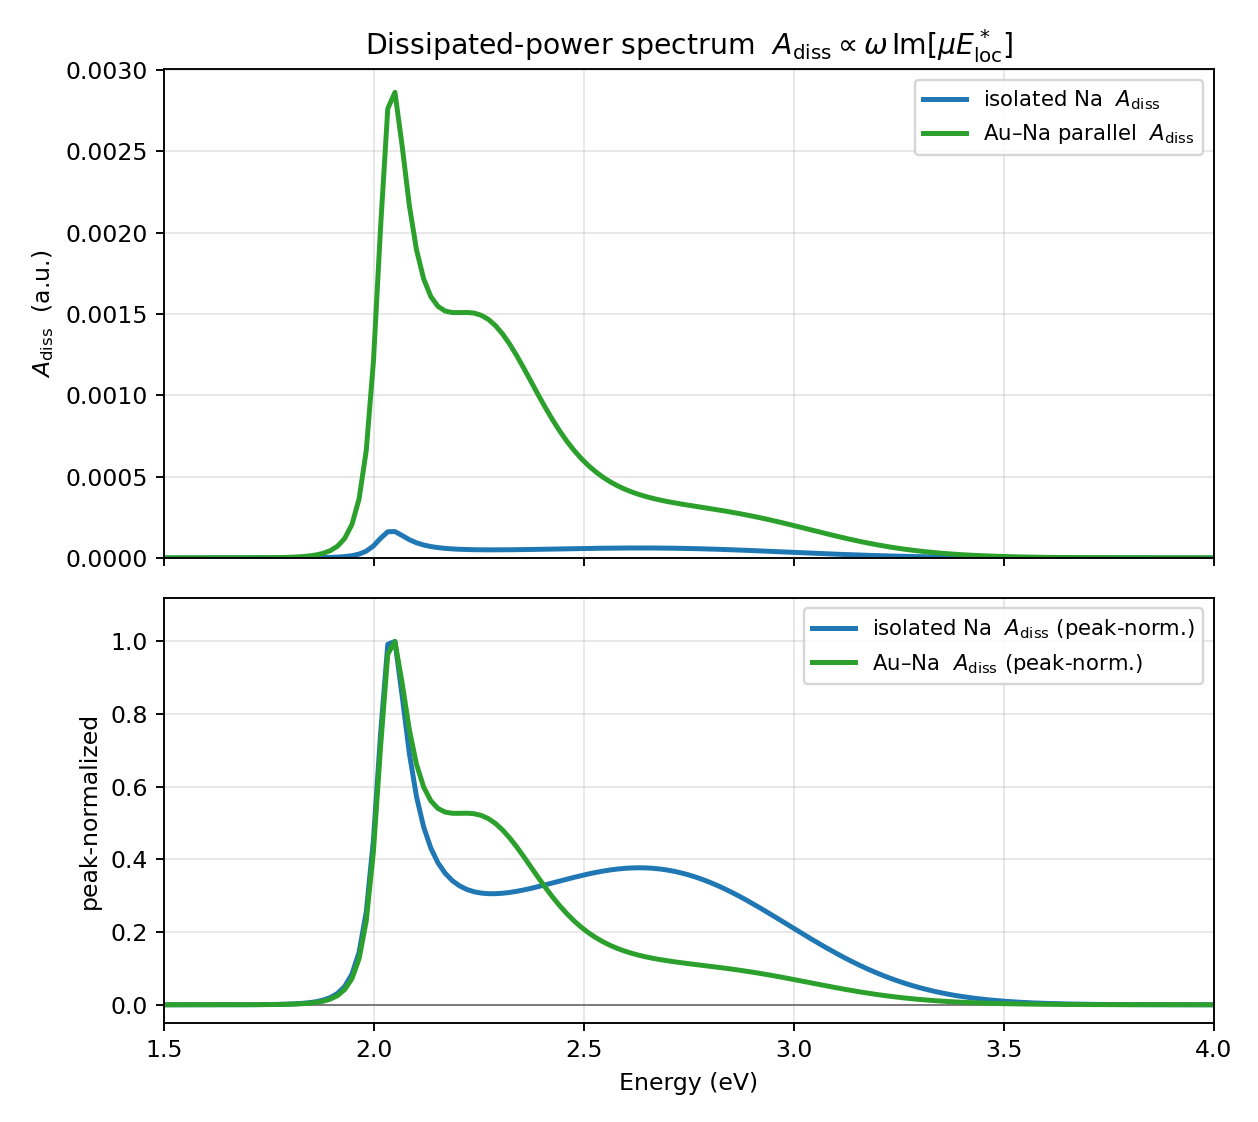
\includegraphics[width=0.88\textwidth]{absorption_dissipated.png}
  \caption{$\Adiss$ from~\eqref{eq:Adiss} for Au--Na parallel (green) and from~\eqref{eq:Adiss-iso} for isolated Na (blue). Top: un-normalized. Bottom: peak-normalized. Isolated Na still carries $\lvert\Einc\rvert^{2}$; the hybrid extra height and the $2.2\,\mathrm{eV}$ shoulder come from $\lvert\Eloc\rvert^{2}$.}
  \label{fig:Adiss}
\end{figure}

\noindent
In order to remove the peak shoulder seen in $A_{\text{diss}}^{\text{iso}}$, we should divide by the squared incident field, but doing so would give us a new quantity: molecular absorption cross section.
That ratio is most cleanly written after introducing the local-field factor $G$.\\

\subsection{Local field enhancement}
\label{sec:G}

\noindent
The complex local-field factor is
\begin{equation}
  G(\om)
  :=
  \frac{\Eloc(\om)}{\Einc(\om)}.
  \label{eq:G}
\end{equation}
Isolated Na would have \(\Eloc(\om)=\Einc(\om)\) so $G=1$.
The shared delay phase of the pulse drops out of $\Eloc/\Einc$, so the structure left in $G$ is the scattering from the NP.\\

\begin{figure}[H]
  \centering
  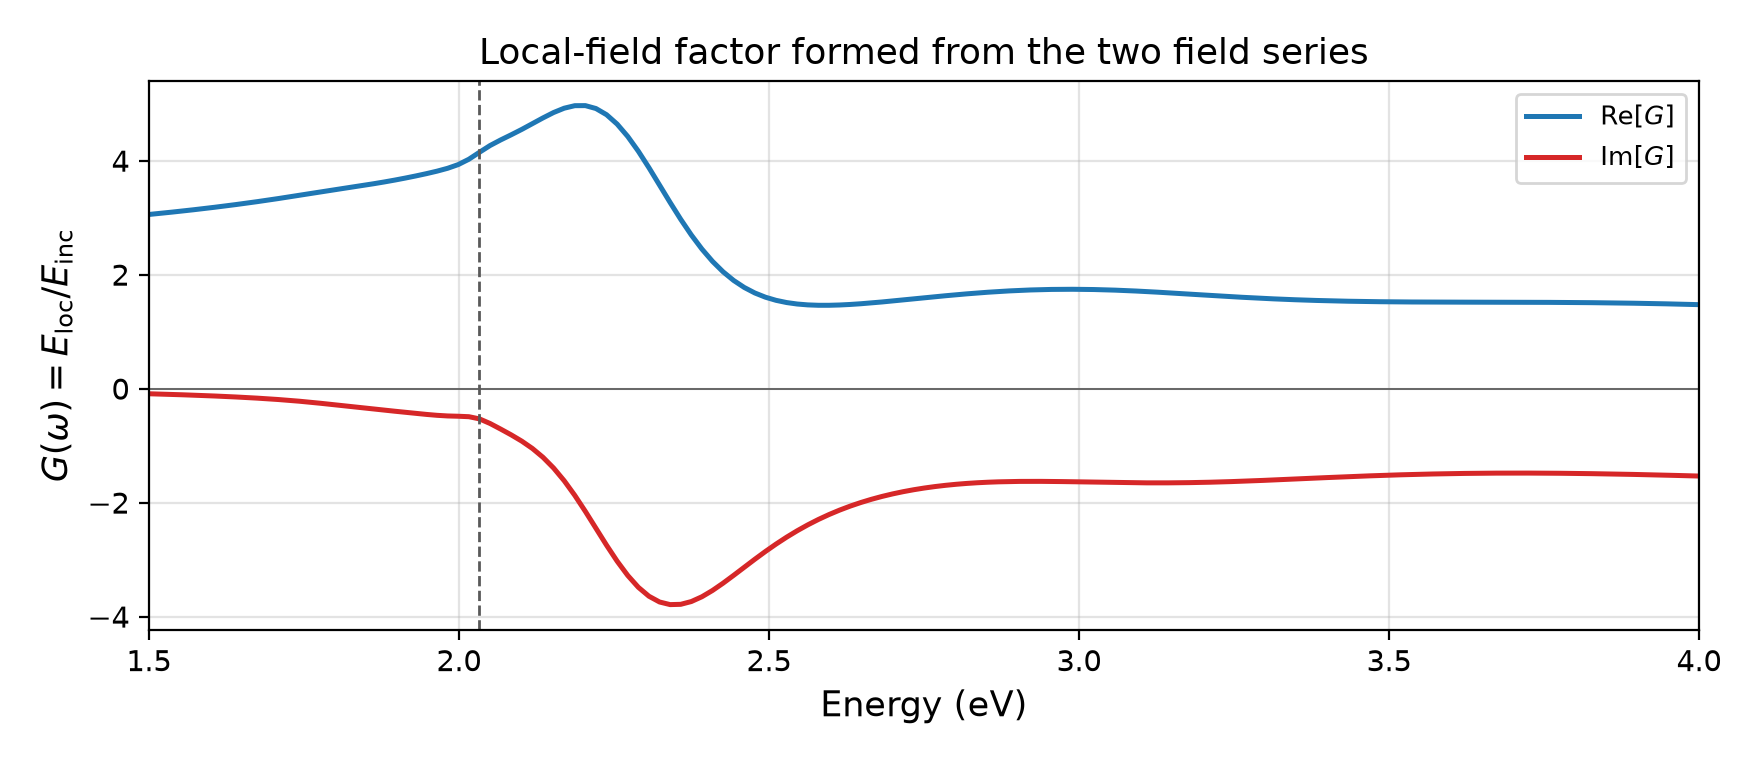
\includegraphics[width=0.92\textwidth]{series_G.png}
  \caption{Local-field factor $G=\Eloc/\Einc$. Dashed line: Na resonance.}
  \label{fig:series-G}
\end{figure}

\noindent
We can then rewrite~\eqref{eq:mu} in terms of \(G(\om)\):
\begin{equation}
    \frac{\mu(\om)}{\Einc(\om)} = \alpm(\om)G(\om)
\end{equation}
and if we define $\alpeff(\om) := \alpm(\om)G(\om)$,
\begin{equation}
  \mu(\om) = \alpeff(\om)\Einc(\om).
  \label{eq:two-ratios}
\end{equation}
So, $\alpeff$ is the molecular dipole expressed in the incident field. The molecule still responds to $\Eloc$; $\alpeff = \alpm G$ is that response as seen from the source.
The extra height of hybrid $\Adiss$ is $\lvert G\rvert^{2}$: $\lvert\Eloc\rvert^{2}=\lvert G\rvert^{2}\lvert\Einc\rvert^{2}$, and $\lvert G(2.03\,\mathrm{eV})\rvert^{2}\approx 17.7$.\\

% =============================================================================
\subsection{\texorpdfstring{Molecular absorption cross section $\sigmol$}{Molecular absorption cross section sigma\_mol}}
\label{sec:sigma}
% =============================================================================

\noindent
A cross section is power over incident flux.
A plane wave in Gaussian units has time-averaged Poynting intensity~\cite{jackson1999}
\begin{equation}
  I_{\mathrm{inc}}
  =
  \frac{c}{8\pi}\lvert\tilde E_{\mathrm{inc}}\rvert^{2},
  \label{eq:I}
\end{equation}
and, for the pulse, the same object built from the DFT of the vacuum reference,
\begin{equation}
  I_{\mathrm{inc}}(\om)
  =
  \frac{c}{8\pi}\lvert\Einc(\om)\rvert^{2}.
  \label{eq:Iw}
\end{equation}
The molecular absorption cross section referred to the vacuum wave in~\eqref{eq:Iw} is
\begin{equation}
  \sigmol(\om)
  :=
  \frac{\overline{P}(\om)}{I_{\mathrm{inc}}(\om)}
  =
  \frac{4\pi\om}{c}
  \frac{\im{\mu(\om)\Eloc^{\ast}(\om)}}{\lvert\Einc(\om)\rvert^{2}}.
  \label{eq:sigmol}
\end{equation}
With~\eqref{eq:mu} and $\Eloc=G\Einc$ this is
\begin{equation}
  \sigmol(\om)
  =
  \frac{4\pi\om}{c}
  \im{\alpm(\om)}
  \lvert G(\om)\rvert^{2}.
  \label{eq:sigmol-G}
\end{equation}
The effect of the nanoparticle enters from $\lvert G\rvert^{2}$.
A passive molecule (one with no significant emission back into the system) has $\im{\alpm}\ge 0$, so $\sigmol\ge 0$.\\

\begin{figure}[H]
  \centering
  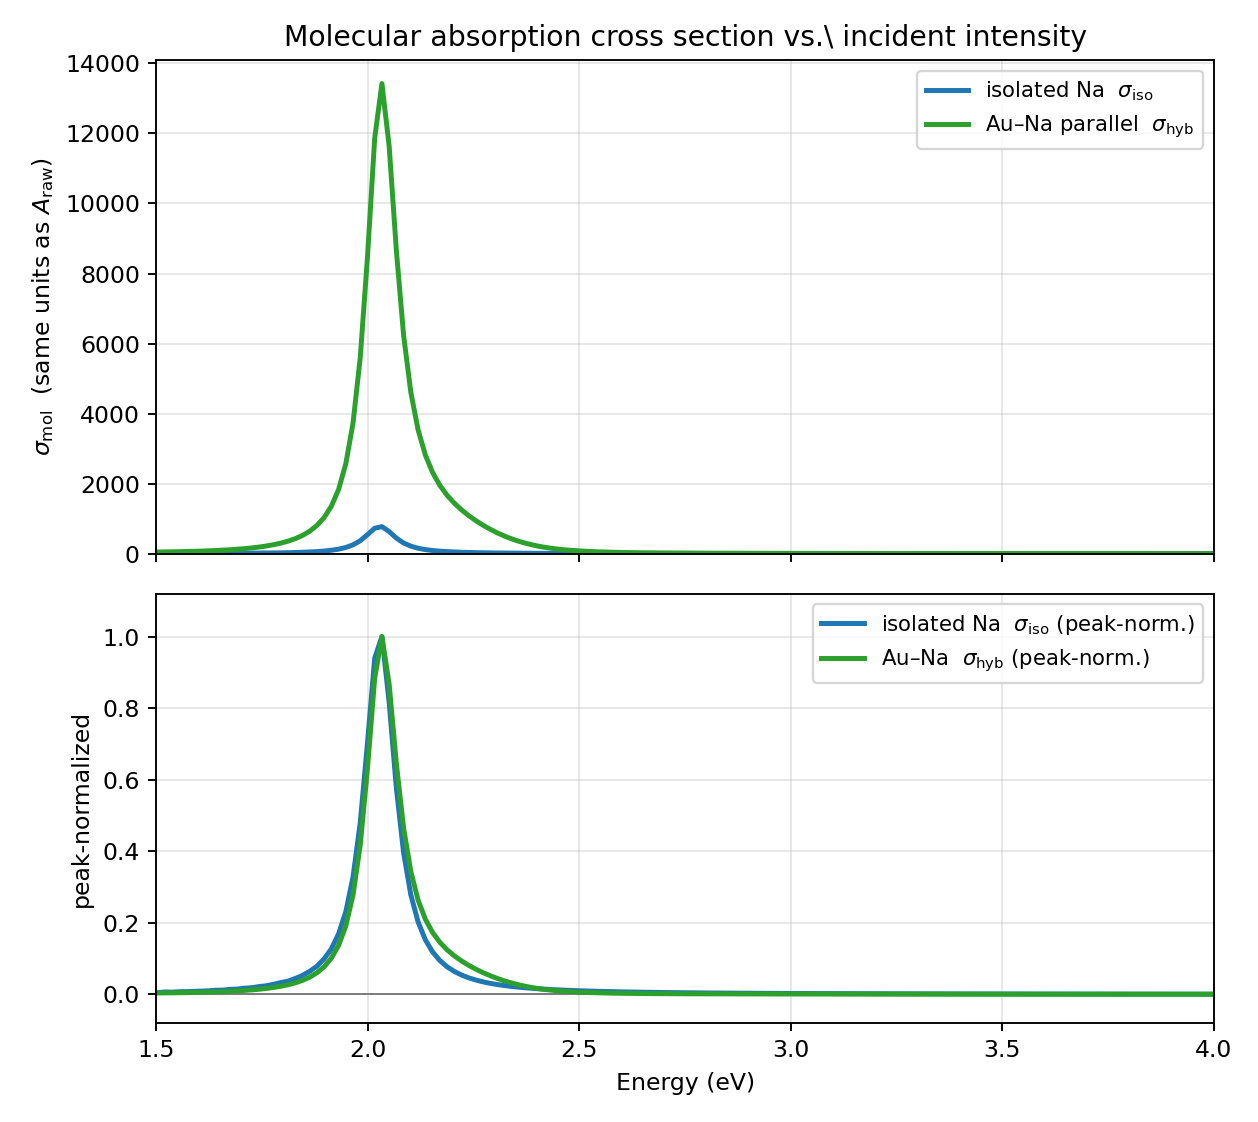
\includegraphics[width=0.78\textwidth]{absorption_cross_section.png}
  \caption{$\sigmol$ for Au--Na parallel (green) and isolated Na (blue). Top: un-normalized. Bottom: peak-normalized.}
  \label{fig:sigma}
\end{figure}

\subsection{Peak-normalized difference of the two cross sections}
\label{sec:sigma-diff}

\noindent
After peak-normalization the two curves in Figure~\ref{fig:sigma} look almost the same, but they are not identical.
Normalizing each spectrum to its own maximum strips the overall $\lvert G\rvert^{2}$ height (the hybrid peak is $\approx 17.7$ times the isolated peak) so the residual lineshape mismatch is visible.
Both maxima sit at $2.033\,\mathrm{eV}$.
The difference
\begin{equation}
  \Delta(E)
  =
  \frac{\sigmol^{\mathrm{hyb}}(E)}{\sigmol^{\mathrm{hyb,\,max}}}
  -
  \frac{\sigmol^{\mathrm{iso}}(E)}{\sigmol^{\mathrm{iso,\,max}}}
  \label{eq:sigma-diff}
\end{equation}
is therefore zero at $2.033\,\mathrm{eV}$ by construction (Figure~\ref{fig:sigma-diff}).
The leftover is an odd swing across the Na line: $\min\Delta=-0.071$ at $1.999\,\mathrm{eV}$ and $\max\Delta=+0.069$ at $2.084\,\mathrm{eV}$, from the slow rise of $\lvert G(\om)\rvert^{2}$ across the resonance.
The hybrid line is leaner on the red side and heavier on the blue; past $\sim 2.5\,\mathrm{eV}$ the peak-normalized spectra agree to less than $1\%$.\\

\begin{figure}[H]
  \centering
  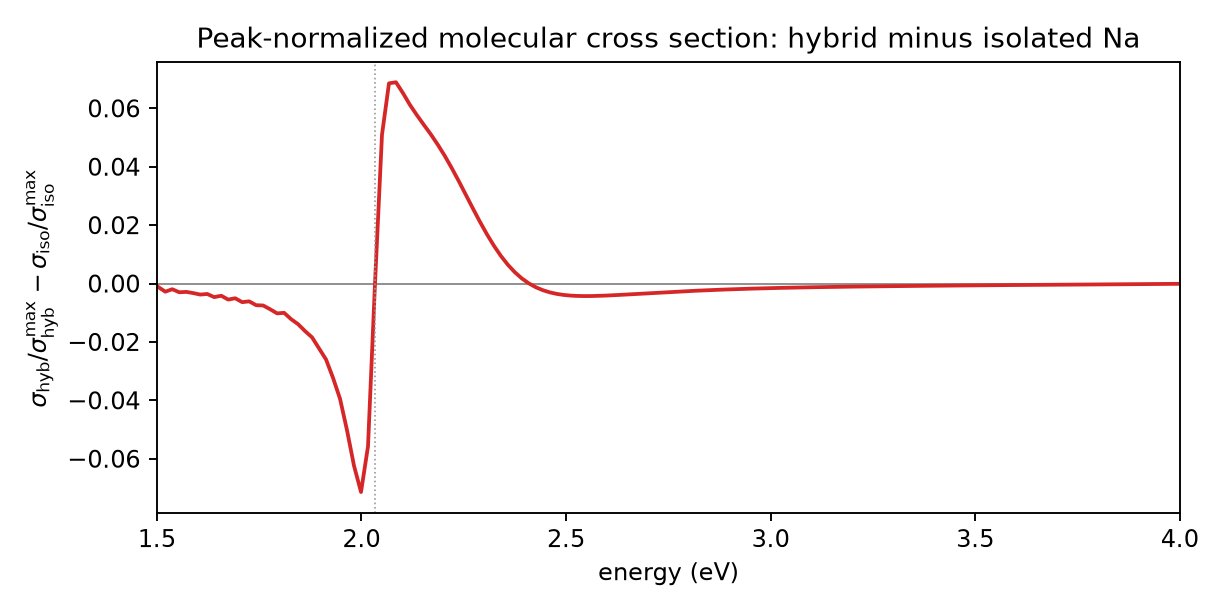
\includegraphics[width=0.88\textwidth]{sigma_mol_peaknorm_difference.png}
  \caption{Peak-normalized hybrid $\sigmol$ minus peak-normalized isolated Na. The dotted line is $2.033\,\mathrm{eV}$. The odd residual is the slow tilt of $\lvert G\rvert^{2}$ across the molecular line, not a second resonance.}
  \label{fig:sigma-diff}
\end{figure}

% =============================================================================
\section{\texorpdfstring{Modified power using $\Einc$}{Modified power using E\_inc}}
\label{sec:transition}
% =============================================================================
\subsection{\texorpdfstring{Why refer the same dipole to $\Einc$}{Why refer the same dipole to E\_inc}}

\noindent
Both $\Adiss$ and $\sigmol$ are built from the field that actually sits on the atom, so they answer how much the molecule absorbs.
They cannot tell us how that absorption appears to the incoming wave: $\Eloc$ already contains the nanoparticle, and dividing by it (or contracting with it) removes the phase of the gap field.
The experimentally controlled quantity is the incident pulse $\Einc$.\\

\noindent
$\Eloc$ tells us what the molecule is.
$\Einc$ tells us what the hybrid setup does to the light we sent.
An optical experiment does not have a probe in the $1.45\mathrm{nm}$ gap; it knows the wave that was launched.
A Gersten--Nitzan model is written in that same field,
\begin{equation}
  \alpeff
  =
  \frac{\alpm G}{1-\alpm S}
  =
  \frac{\mu}{\Einc}.
  \label{eq:GN}
\end{equation}
If we divide $\mu$ by $\Eloc$ we undo the nanoparticle on purpose and recover $\alpm$.
That is a useful check (and it is how one confirms that back-action is weak: $\lvert\alpm^{\mathrm{hyb}}/\alpm^{\mathrm{iso}}\rvert\approx 0.99$ at $2.03\mathrm{eV}$).
It is not a hybrid lineshape.\\

\noindent
The same dipole $\mu(t)$, referred to $\Einc$ instead of $\Eloc$, is therefore the molecular response as seen from the source.
We form it first as a bookkeeping analogue of~\eqref{eq:Pt},
\begin{equation}
  P_{\mathrm{inc}}(t)
  =
  \dot{\mu}(t)\Einc(t),
  \label{eq:Pinc-t}
\end{equation}
which is \emph{not} the mechanical power into the atom.
It is~\eqref{eq:Pt} with the partner field replaced by the vacuum wave.
% The cycle average and the spectral density are the same algebra as Section~\ref{sec:cycle},
\begin{equation}
  \overline{P}_{\mathrm{inc}}(\om)
  =
  \frac{\om}{2}
  \im{\mu(\om)\Einc^{\ast}(\om)}.
  \label{eq:Pinc}
\end{equation}
Dividing by the incident intensity~\eqref{eq:Iw} and using
\begin{equation}
  \frac{\mu\Einc^{\ast}}{\lvert\Einc\rvert^{2}}
  =
  \frac{\mu}{\Einc}
  \label{eq:ratio-id}
\end{equation}
gives
\begin{equation}
  \Ainc(\om)
  :=
  \frac{\overline{P}_{\mathrm{inc}}(\om)}{I_{\mathrm{inc}}(\om)}
  =
  \frac{4\pi\om}{c}
  \im{\frac{\mu(\om)}{\Einc(\om)}}
  =
  \frac{4\pi\om}{c}
  \im{\alpeff(\om)}.
  \label{eq:Ainc}
\end{equation}
This is the vacuum dipole formula~\cite{jackson1999} with $\alpha\mapsto\alpeff$ and $E\mapsto\Einc$.

% =============================================================================
\subsection{\texorpdfstring{The driver spectrum $\Araw$}{The driver spectrum A\_raw}}
\label{sec:Araw}
% =============================================================================

\noindent
PlasMol plots~\eqref{eq:Ainc} with a global minus so that a physical $3s\to 3p$ peak points up.
With the DFT~\eqref{eq:dft}, $\im{\mu/\Einc}$ is negative at a passive Lorentzian, and
\begin{equation}
  \Araw(\om)
  =
  -\frac{4\pi\om}{c}
  \im{\frac{\mu(\om)}{\Einc(\om)}}
  =
  -\frac{4\pi\om}{c}
  \im{\alpeff(\om)}
  \label{eq:Araw}
\end{equation}
is the upright copy of $\Ainc$.
After peak-normalization, $\Araw$ and $\Ainc$ are the same curve up to that sign.
In the code, $\om$ on the prefactor is the energy axis in eV while $c$ is $c_{\mathrm{au}}$, so the absolute scale is not a clean $\mathrm{a.u.}^{2}$ cross section; only the shape is used.\\

\noindent
Expanding the imaginary part,
\begin{equation}
  \im{\alpeff}
  =
  \im{\alpm G}
  =
  \im{\alpm}\re{G}
  +
  \re{\alpm}\im{G}.
  \label{eq:split-im}
\end{equation}
The first term is the even Lorentzian, weighted by $\re{G}$.
The second is the odd (dispersive) wing of $\alpm$ weighted by the phase of the near field.
A Lorentzian model (Figure~\ref{fig:alpha-re-im}) has $\re{\alpm}>0$ below $\om_m=2.033\mathrm{eV}$, $0$ on resonance, and $\re{\alpm}<0$ above it.
As soon as $\im{G}\neq 0$, the second term goes negative on the blue side and can overcome the Lorentzian.
That product is the lobe at $2.32\mathrm{eV}$ in Figure~\ref{fig:Araw}.
Isolated Na has $\im{G}\simeq 0$, so $\Araw$ stays non-negative.
The delay beating of Figure~\ref{fig:series-ft} cancels in the ratio $\mu/\Einc$; what remains is $\alpeff$, whose imaginary part (sign-flipped) is $\Araw$.\\

\begin{figure}[H]
  \centering
  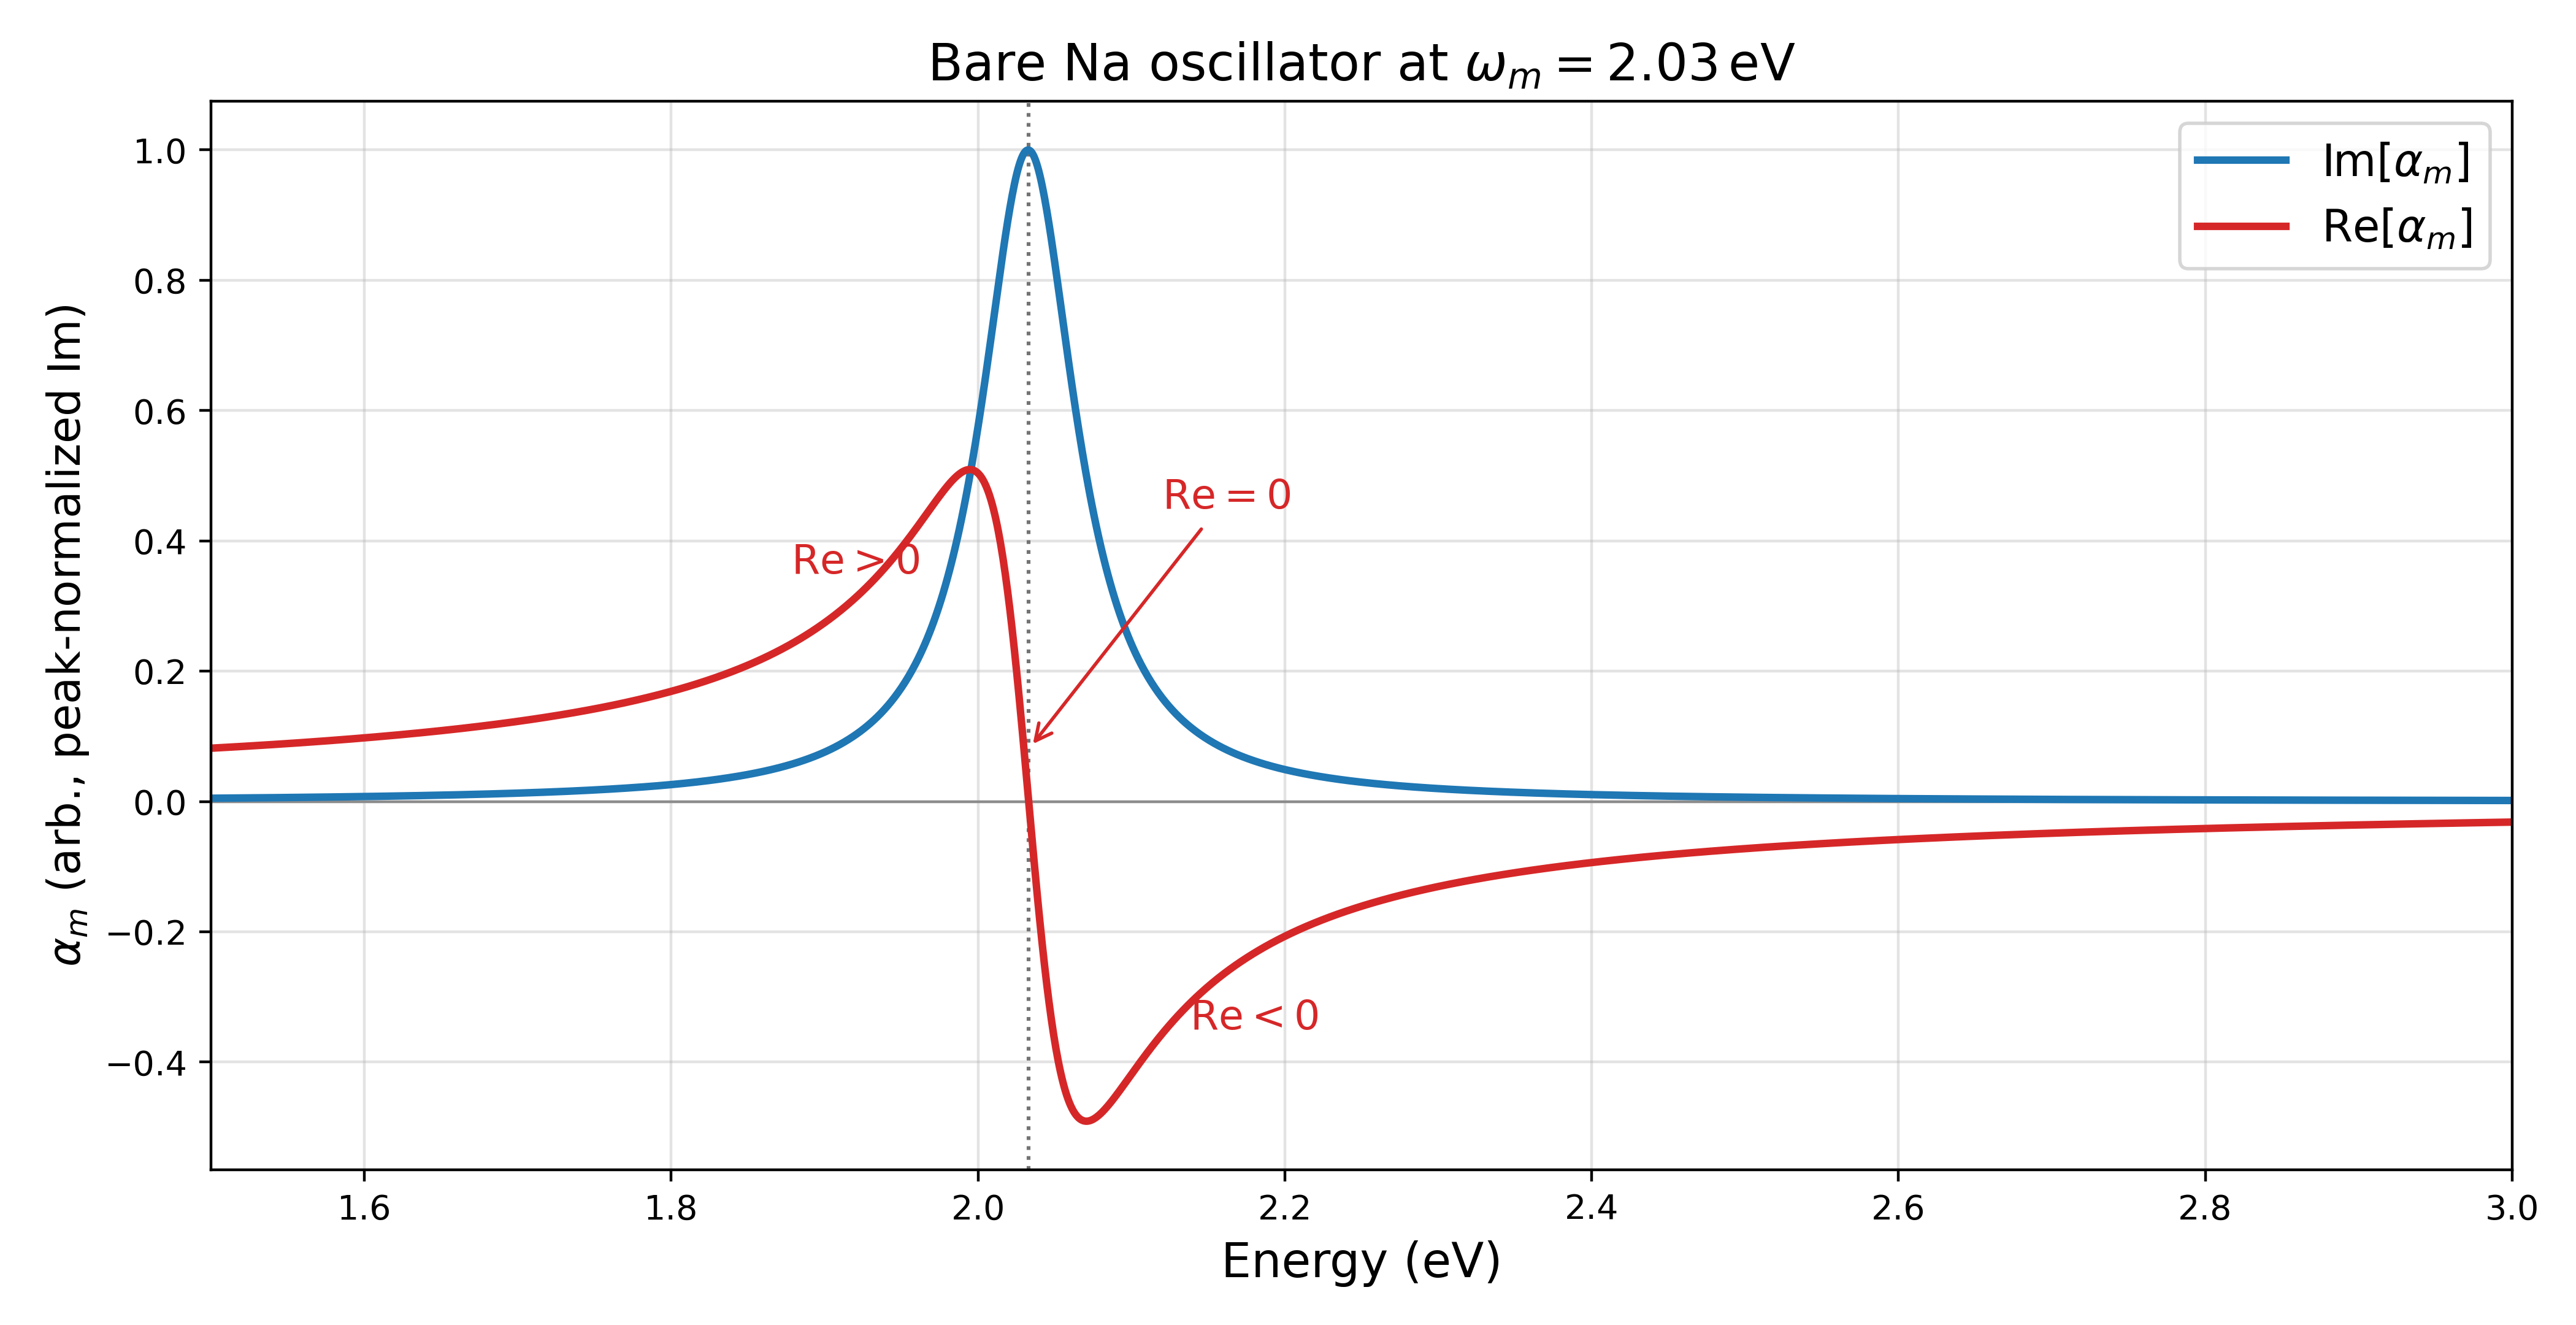
\includegraphics[width=0.72\textwidth]{alpha_re_im.png}
  \caption{Model $\re{\alpm}$ (red, odd) and $\im{\alpm}$ (blue, even) about $2.033\mathrm{eV}$. The red wing is what $\im{G}$ multiplies in~\eqref{eq:split-im}.}
  \label{fig:alpha-re-im}
\end{figure}

\begin{figure}[H]
  \centering
  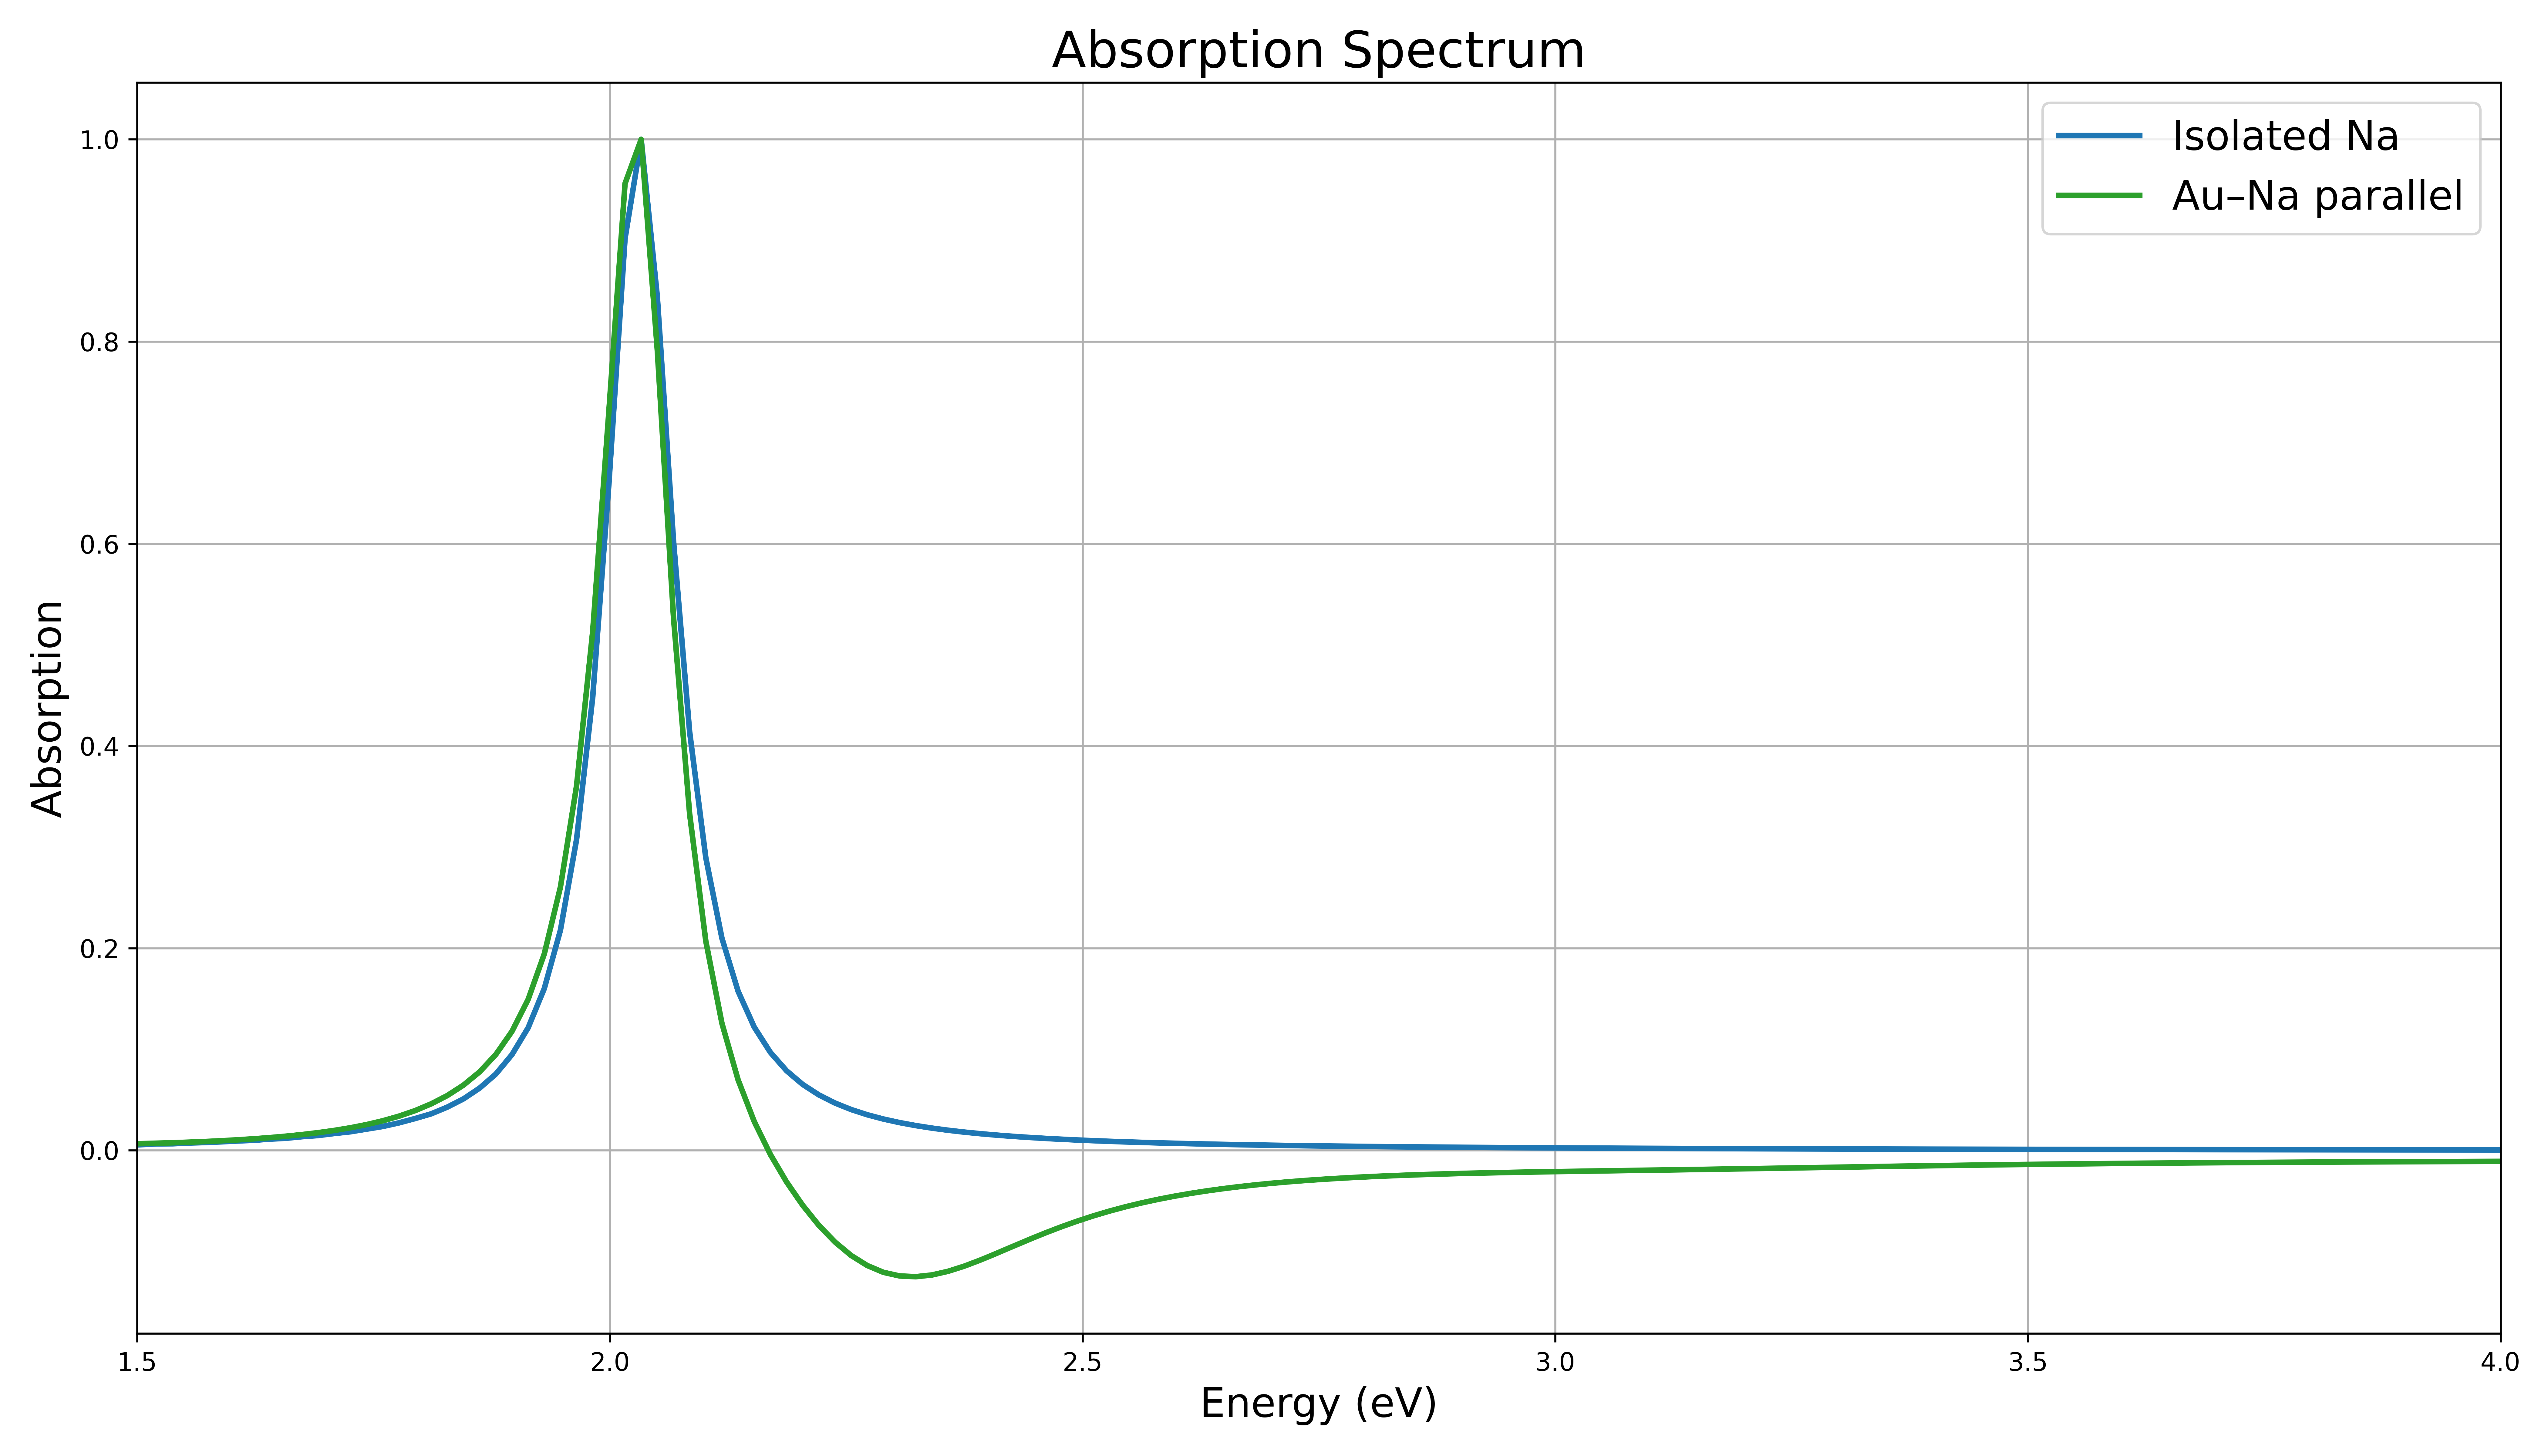
\includegraphics[width=0.88\textwidth]{spectrum_parallel_vs_na_ref.png}
  \caption{Peak-normalized $\Araw$ for Au--Na parallel (green) and isolated Na (blue), $1.5$--$4.0\mathrm{eV}$. The hybrid curve crosses zero at $2.17\mathrm{eV}$ and reaches $\approx -0.125$ at $2.32\mathrm{eV}$.}
  \label{fig:Araw}
\end{figure}

\noindent
$\mu$ in~\eqref{eq:Araw} is still only the atom.
$\Araw$ is not the extinction of Au+Na, and it is not $\operatorname{Im}[\mathbf{p}_{\mathrm{tot}}/\Einc]$.
It is the molecular dipole expressed in the only field an experiment or a classical hybrid model actually knows.\\

% =============================================================================
\section{The three observables together}
\label{sec:compare}
% =============================================================================

\noindent
The same three time series produce three different spectra, in the order they were derived (Figure~\ref{fig:three}),
\begin{align}
  \Adiss(\om)
  &=
  -\frac{4\pi\om}{c}
  \im{\mu(\om)\Eloc^{\ast}(\om)},
  \label{eq:summary-diss}\\[0.4em]
  \sigmol(\om)
  &=
  \frac{4\pi\om}{c}
  \frac{\im{\mu(\om)\Eloc^{\ast}(\om)}}{\lvert\Einc(\om)\rvert^{2}}
  =
  \frac{4\pi\om}{c}
  \im{\alpm(\om)}
  \lvert G(\om)\rvert^{2},
  \label{eq:summary-sig}\\[0.4em]
  \Araw(\om)
  &=
  -\frac{4\pi\om}{c}
  \im{\frac{\mu(\om)}{\Einc(\om)}}.
  \label{eq:summary-raw}
\end{align}
They are not three normalizations of one curve.
The split is which field sits next to $\mu$, and whether one then divides by $I_{\mathrm{inc}}$.\\

\begin{figure}[H]
  \centering
  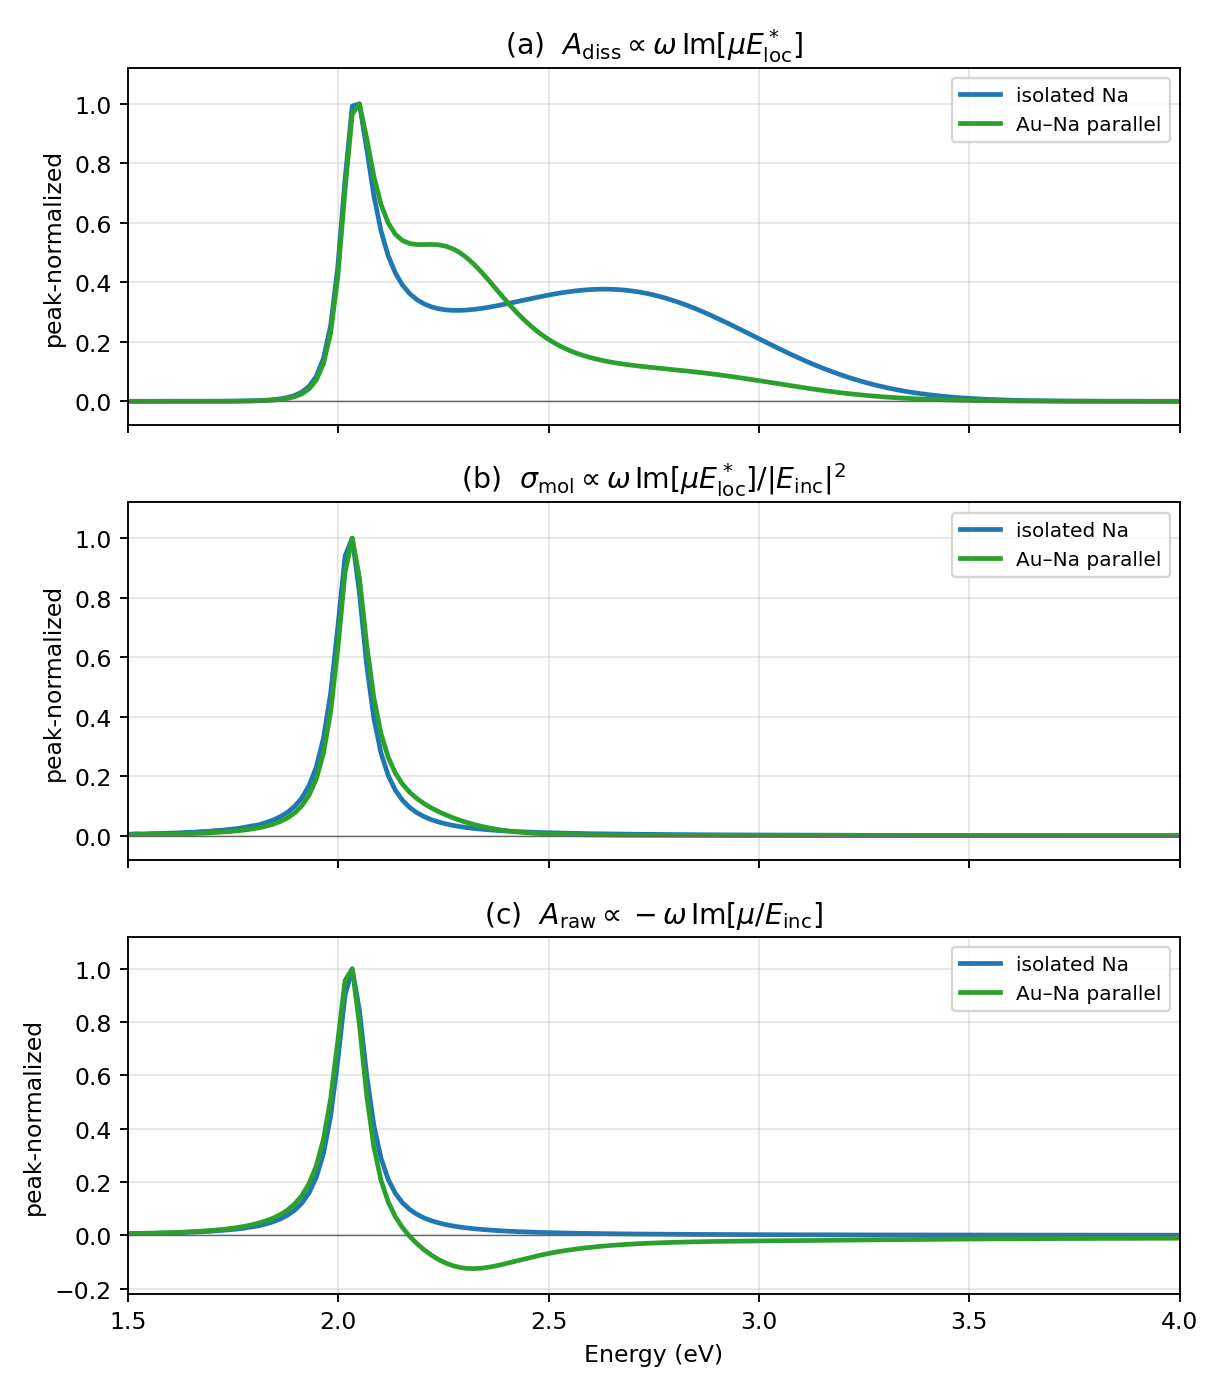
\includegraphics[width=0.92\textwidth]{three_observables.png}
  \caption{Peak-normalized hybrid (green) and isolated-Na (blue) spectra, in the order of Sections~\ref{sec:Adiss}--\ref{sec:Araw}. (a)~$\Adiss$, still carrying $\lvert\Einc\rvert^{2}$ when isolated. (b)~$\sigmol$, the pulse divided out. (c)~$\Araw$; this is the only panel allowed to go negative.}
  \label{fig:three}
\end{figure}

% =============================================================================
\section*{Acknowledgements of convention}
% =============================================================================

\noindent
Phasors follow $e^{-\mathrm{i}\om t}$~\cite{jackson1999}.
The cycle average $\tfrac12\re{\tilde A\tilde B^{\ast}}$ is Jackson \S6.9; the vacuum intensity $c\lvert E\rvert^{2}/8\pi$ is the Gaussian form of \S7.1.
The step from those two formulae to $\sigma=(4\pi\om/c)\im{\alpha}$ is the dipole reduction of the optical theorem, not a single numbered equation in Jackson.
The minus signs in~\eqref{eq:Adiss} and~\eqref{eq:Araw} are DFT bookkeeping, not additional physics.\\

\begin{thebibliography}{9}
\bibitem{jackson1999}
J.~D. Jackson, \emph{Classical Electrodynamics}, 3rd~ed.\ (Wiley, 1999), \S6.9 and \S7.1.
\bibitem{novotny2012}
L.~Novotny and B.~Hecht, \emph{Principles of Nano-Optics}, 2nd~ed.\ (Cambridge University Press, 2012).
\end{thebibliography}

\end{document}
